\section{Contextualização} % (fold)
\label{sec:contextualizacao}

\begin{frame}
    Sistemas com vários itens ou serviços utilizam sistemas
de recomedação. Exemplo:
    \begin{itemize}
        \item Netflix
        \item Amazon
    \end{itemize}
\end{frame}

\begin{frame}
    \begin{itemize}
        \item O Debian possui mais de 49 mil pacotes
        \item A recomendação de pacotes pode ajudar o usuário
        na realização de suas atividades
    \end{itemize}
\end{frame}

% section what_is_solid_ (end)

\section{Problemática} % (fold)
\label{sec:problematica}

\begin{frame}
  \begin{itemize}
    \item Prover uma recomendação útil para o usuário
    \item Entender o contexto temporal do uso de pacotes
  \end{itemize}
\end{frame}

% section s (end)

\section{Objetivo} % (fold)
\label{sec:objetivo}

\begin{frame}
	\say{\textit{Software entities should be open for extension, but closed for modification.}}, \\Meyer, Bertrand
\end{frame}

\begin{frame}


\begin{Parallel}[v]{5cm}{5cm}
    \ParallelLText%
    {
    	\textbf{Bertrand Meyer, 1988}

    	The idea was that once completed, the implementation of a class could only be modified to correct errors.
    }
    \ParallelRText%
    {
    	\textbf{1990s}

    	The implementations can be changed and multiple implementations could be created and polymorphically substituted for each other.
	}
\end{Parallel}

\end{frame}

\begin{frame}

\begin{figure}[h!]
  % \caption{The Extractor inherited.}
  \centering
    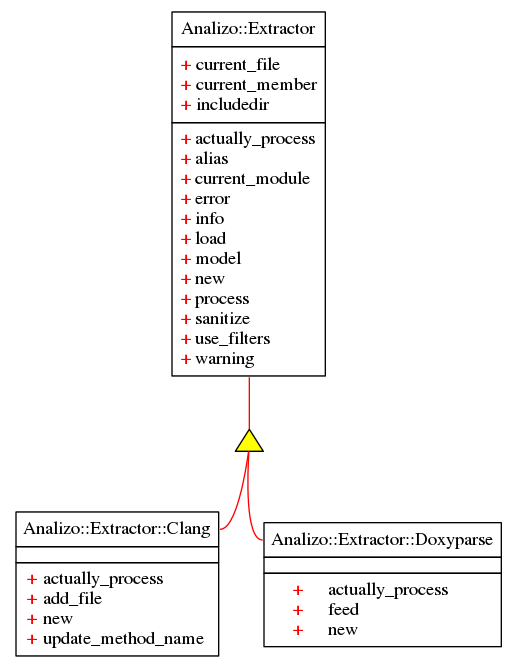
\includegraphics[width=0.5\textwidth]{conteudo/Extractor}
    \caption{Extractor inherited}
\end{figure}

\end{frame}
% subsection use_in_analizo (end)


% section o (end)

\section{Sistemas de recomendação} % (fold)
\label{sec:sistemas_recomendacao}
\begin{frame}
    \say {\textit{Sistemas de recomendação são ferramentas computacionais e
técnicas usadas para produzir recomendação de itens úteis a um
usuário}},\\(MAHMOOD; RICCI, 2009)
\end{frame}

\begin{frame}

\begin{figure}[h!]
  \centering
    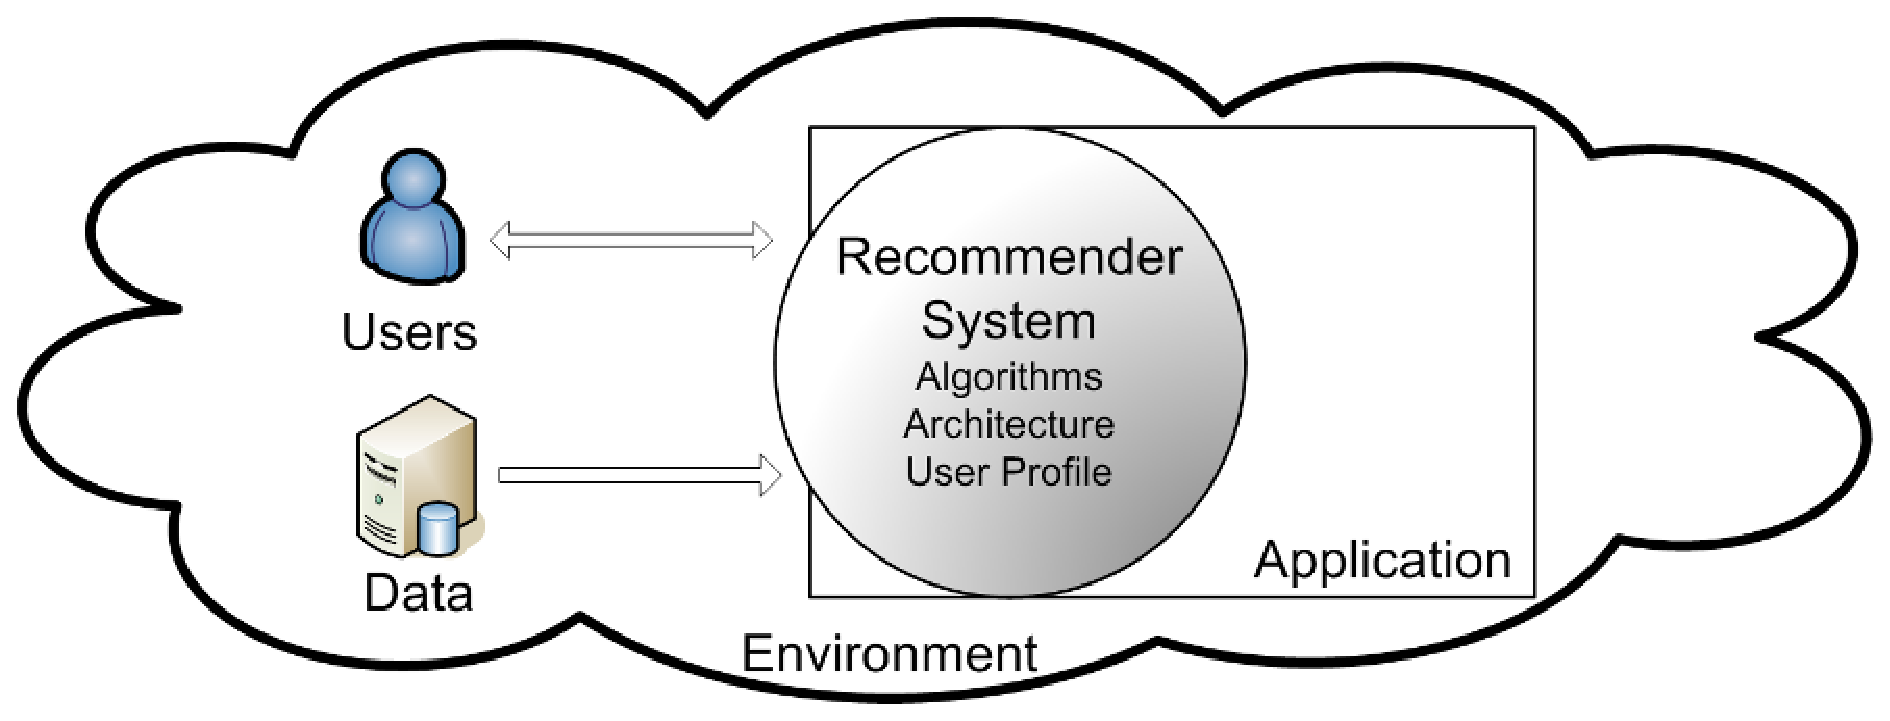
\includegraphics[width=1\textwidth]{figura/recommender_model.eps}
  \caption{Modelo para criação de um sistema de recomendação personalizado (PICAULT et al., 2011)}
\end{figure}

\end{frame}

\begin{frame}
    Tipos de sistemas de recomendação:

    \begin{itemize}
        \item Recomendação baseada em conteúdo
        \item Recomendação colaborativa
        \item Recomendação híbrida
        \item Recomendação por contexto
    \end{itemize}
\end{frame}

\begin{frame}

\begin{figure}[h!]
  \centering
    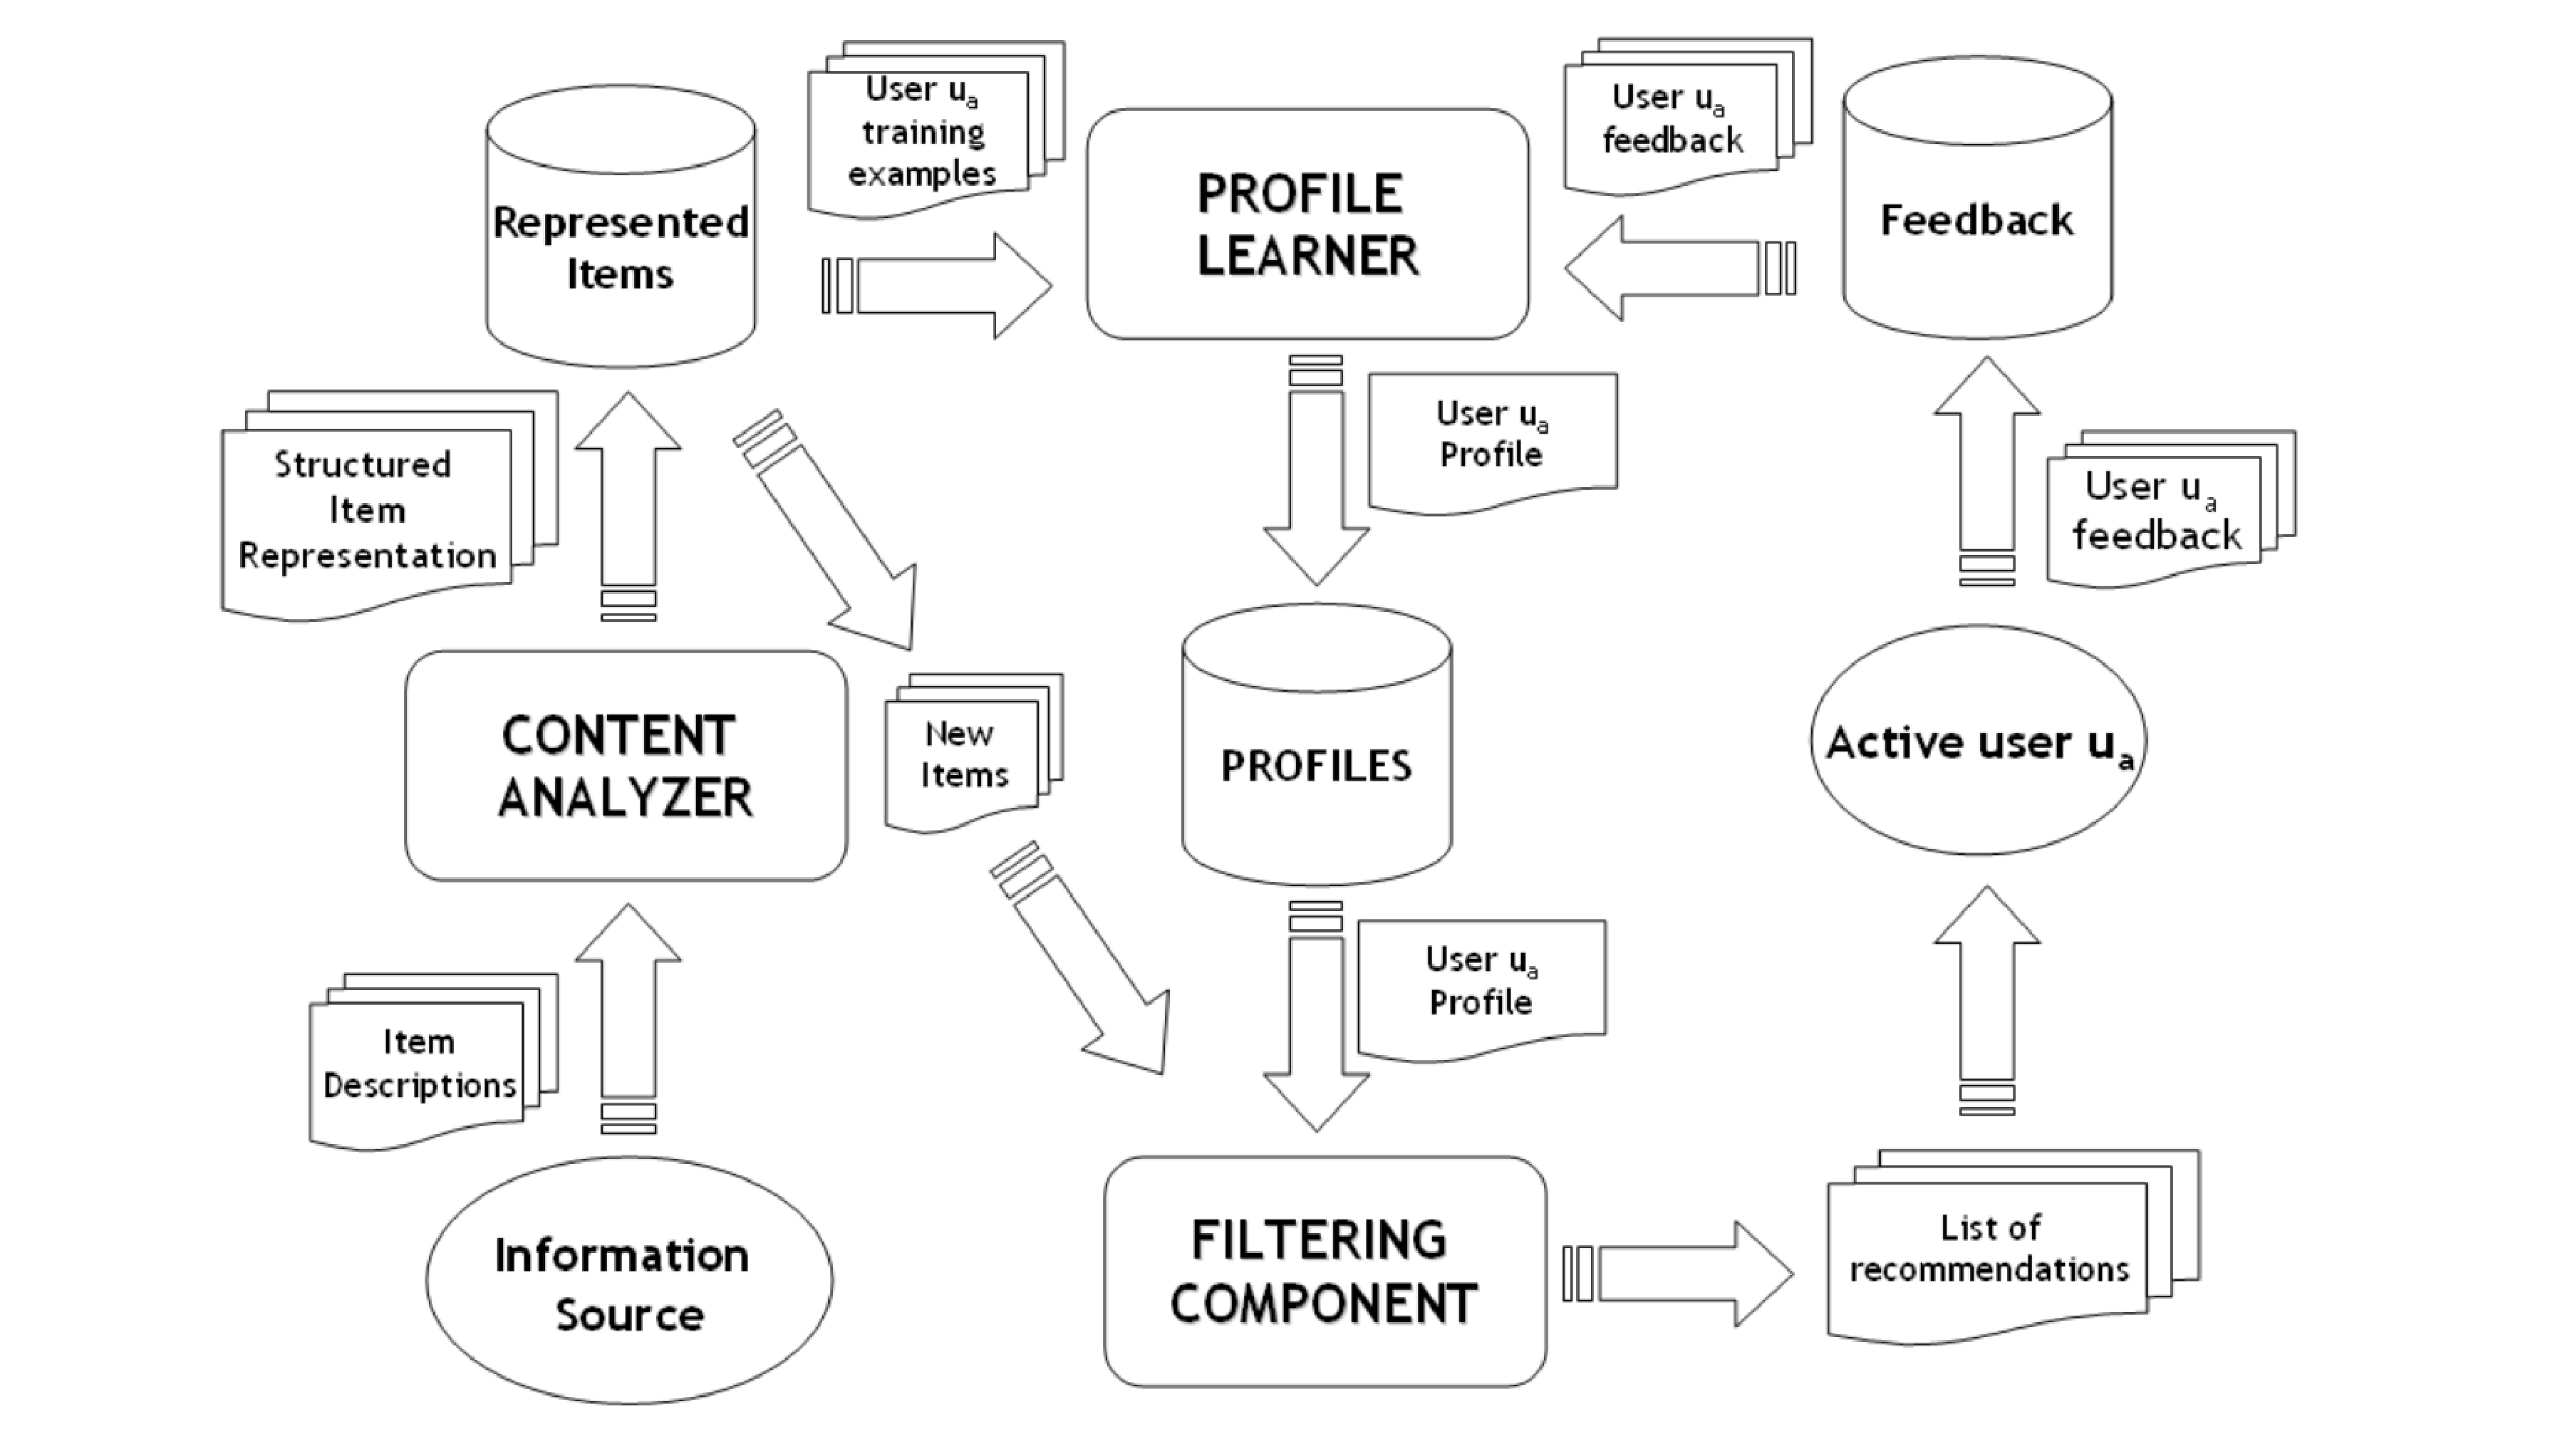
\includegraphics[width=1\textwidth]{figura/recomendacao_conteudo.eps}
  \caption{Fluxo para construção de um sistema de recomendação por conteúdo (LOPS; GEMMIS; SEMERARO, 2011)}
\end{figure}

\end{frame}

\begin{frame}

\begin{figure}[h!]
  \centering
    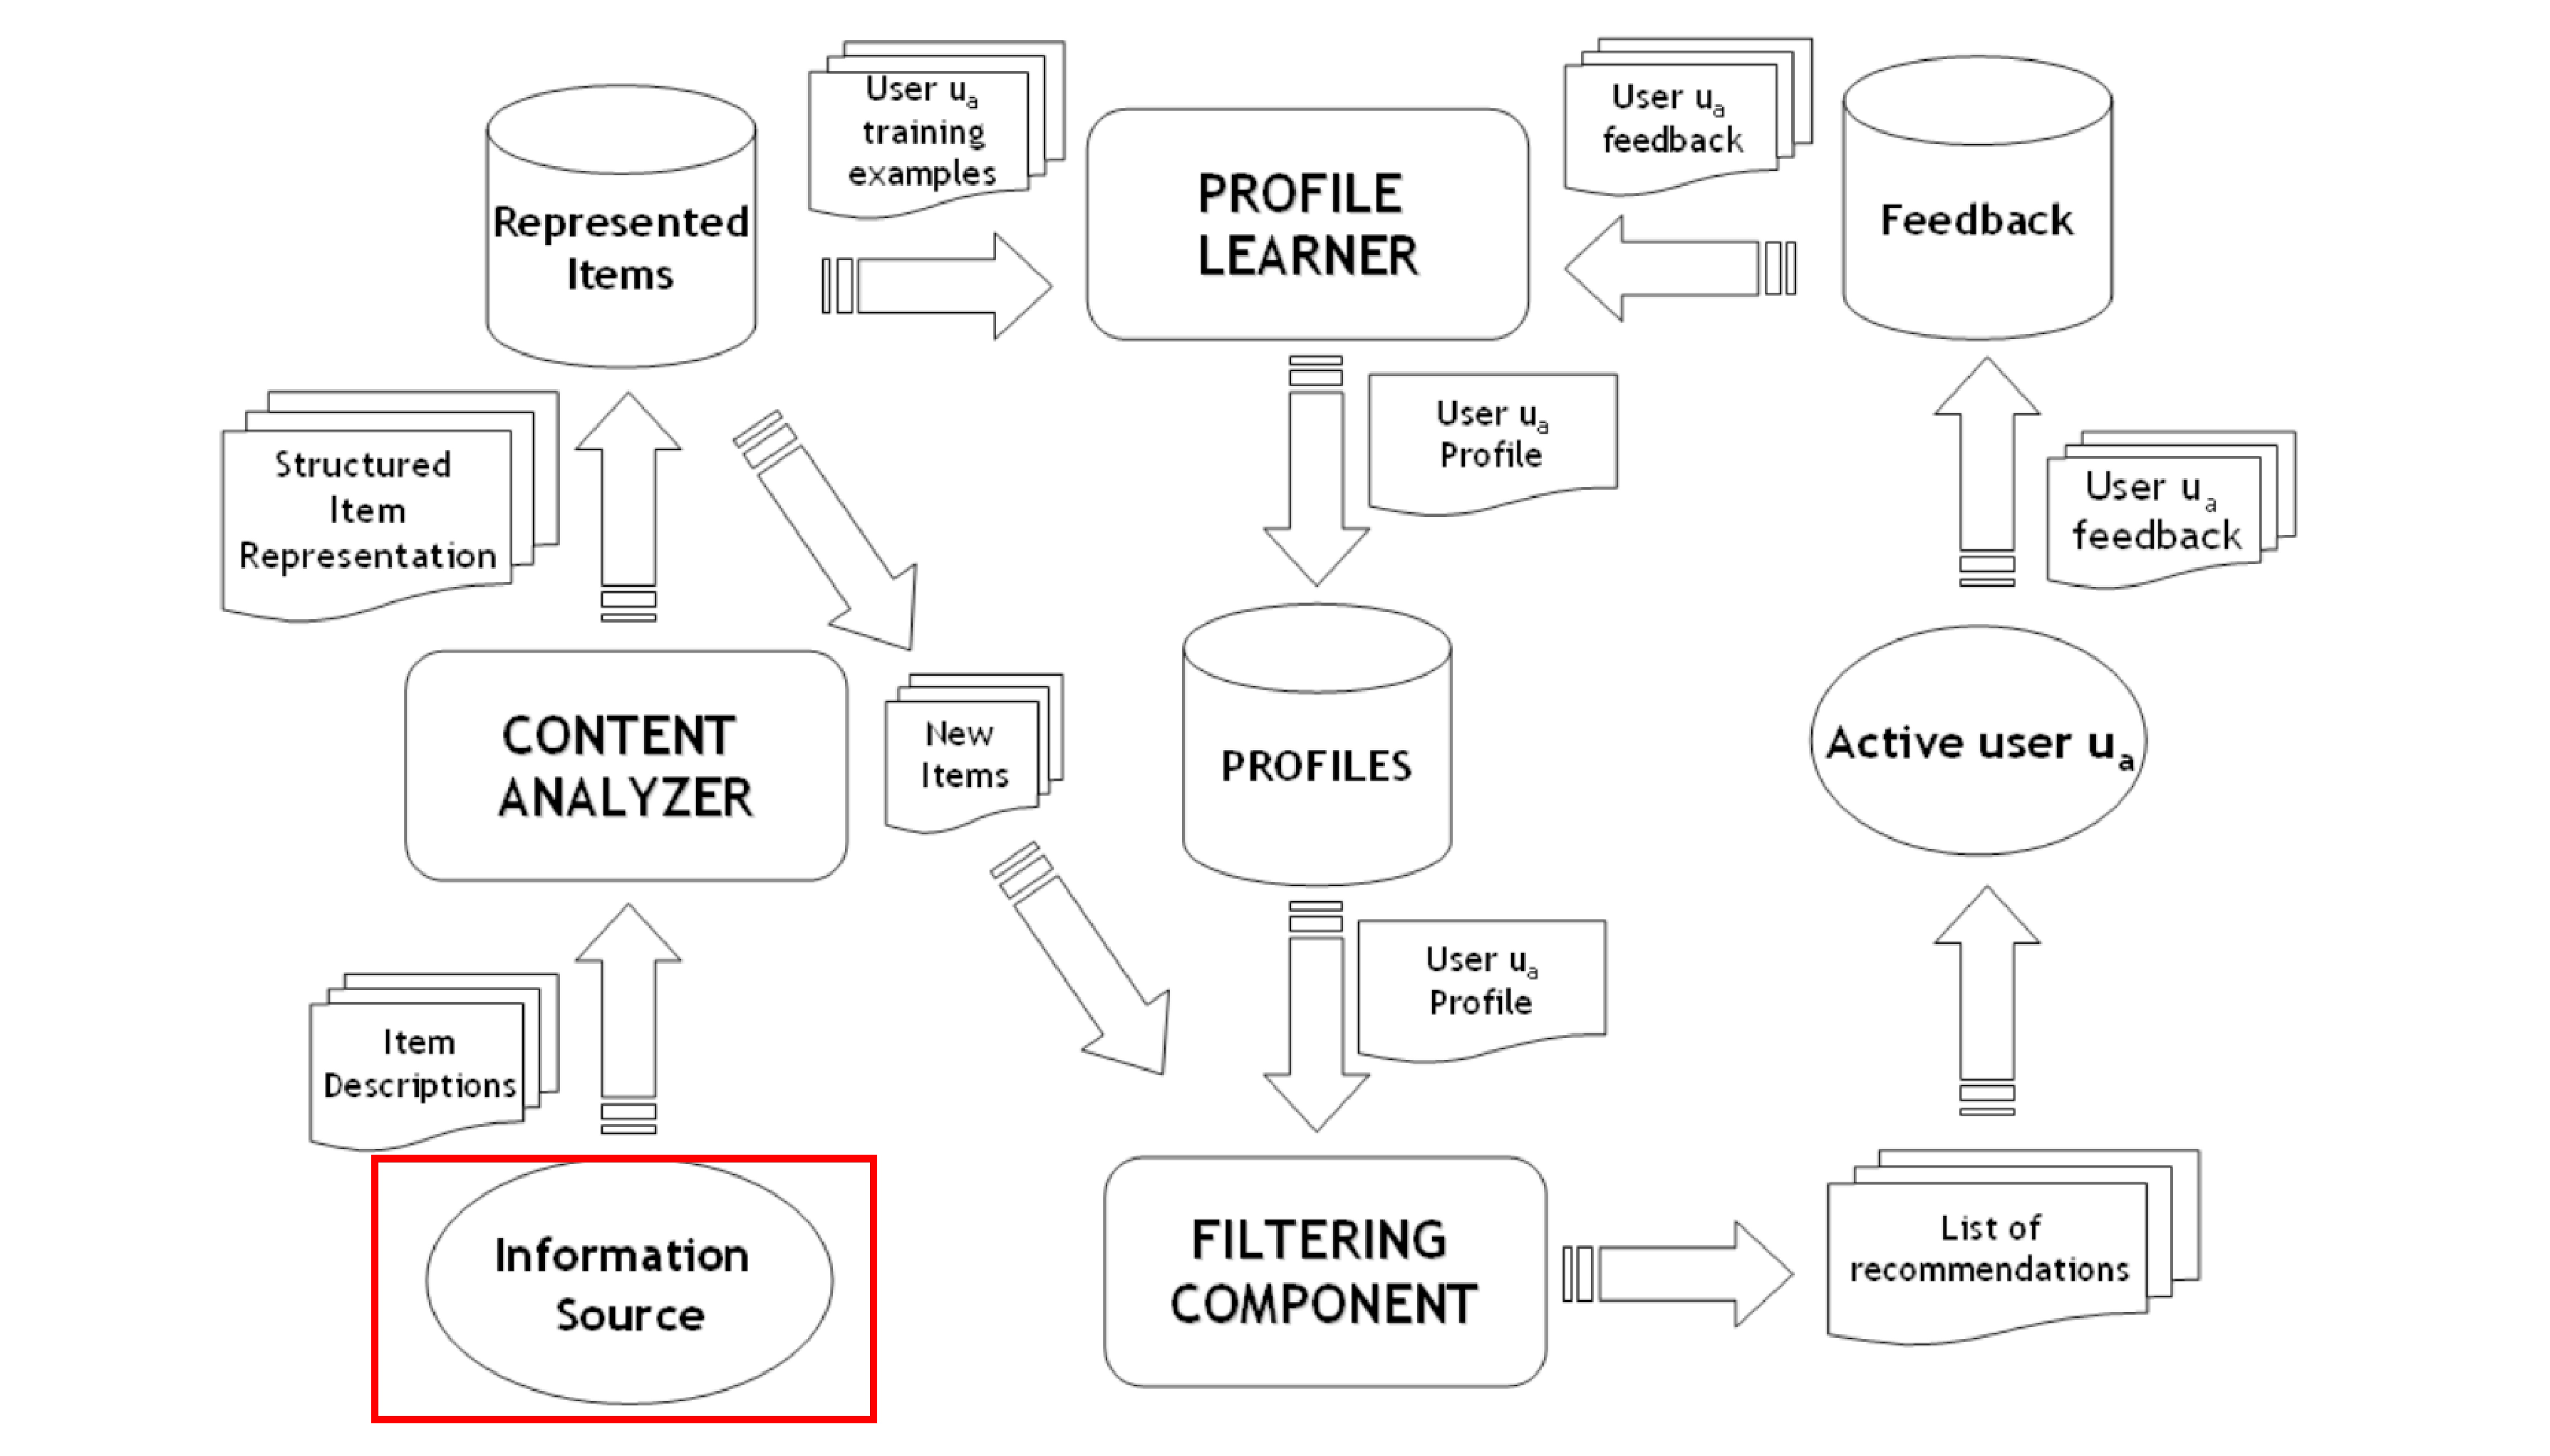
\includegraphics[width=1\textwidth]{figura/recomendacao_conteudo_1.eps}
  \caption{Fluxo para construção de um sistema de recomendação por conteúdo (LOPS; GEMMIS; SEMERARO, 2011)}
\end{figure}

\end{frame}

\begin{frame}

\begin{figure}[h!]
  \centering
    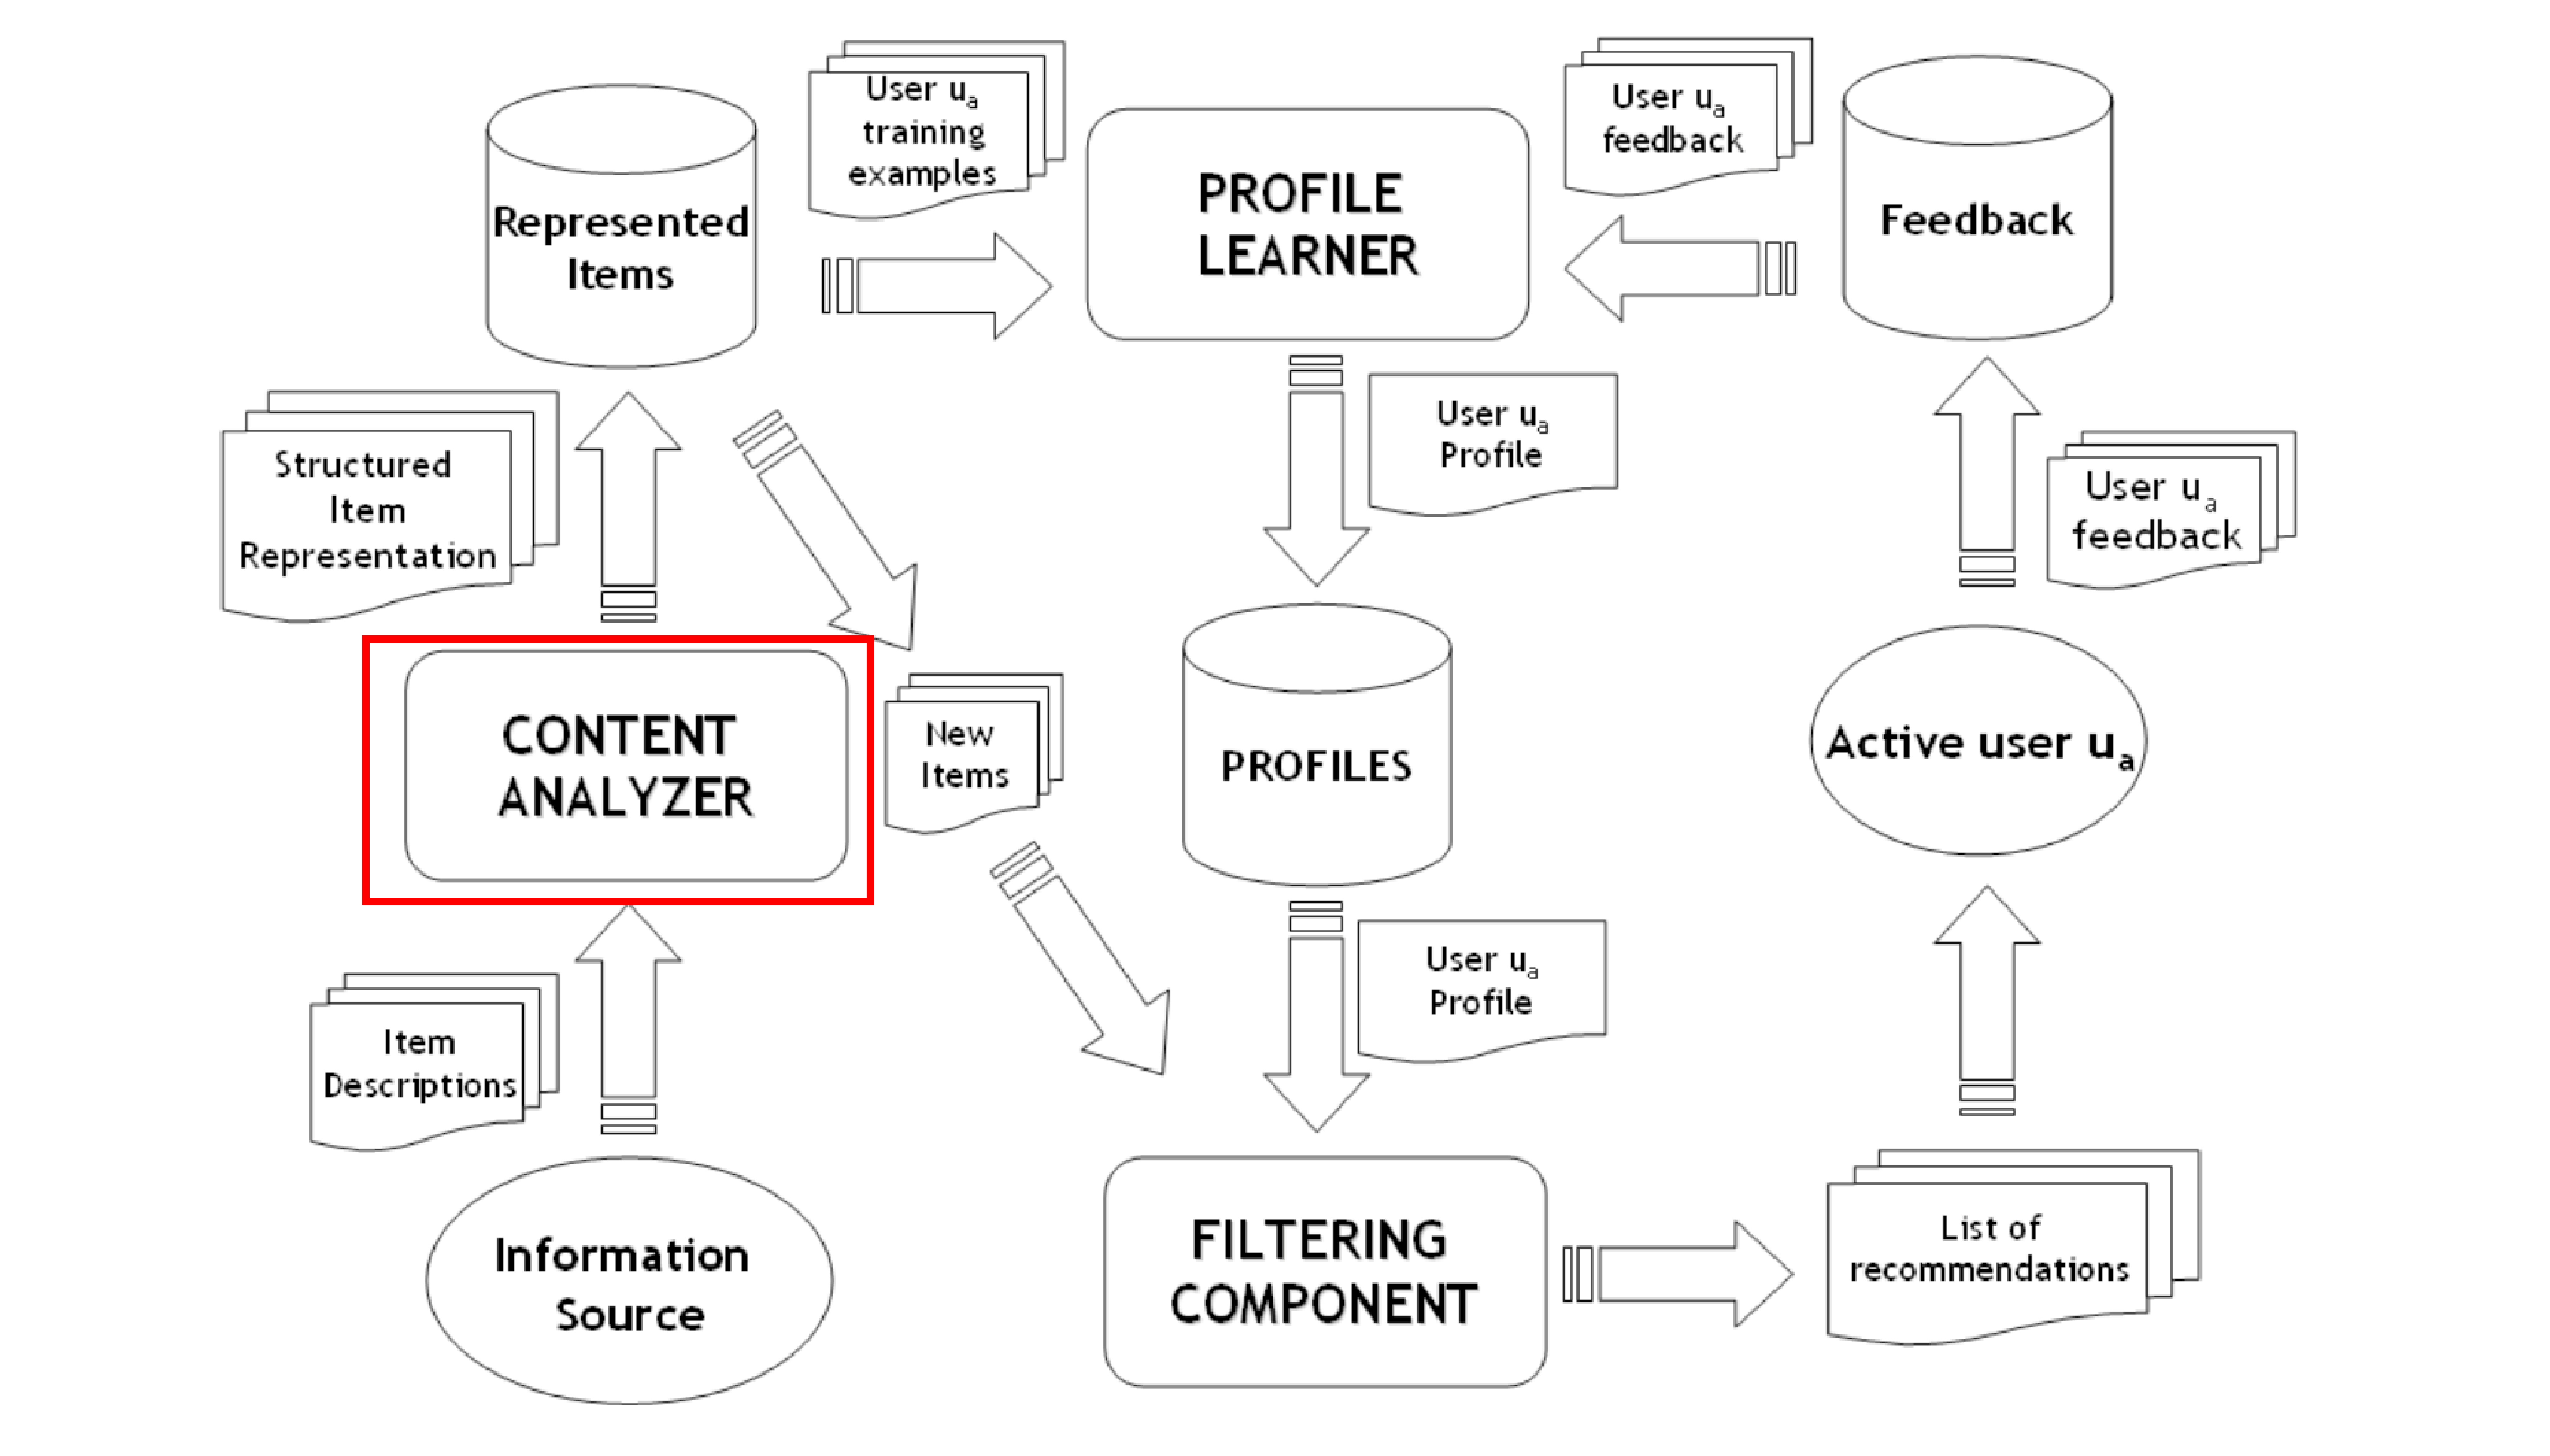
\includegraphics[width=1\textwidth]{figura/recomendacao_conteudo_2.eps}
  \caption{Fluxo para construção de um sistema de recomendação por conteúdo (LOPS; GEMMIS; SEMERARO, 2011)}
\end{figure}

\end{frame}

\begin{frame}

\begin{figure}[h!]
  \centering
    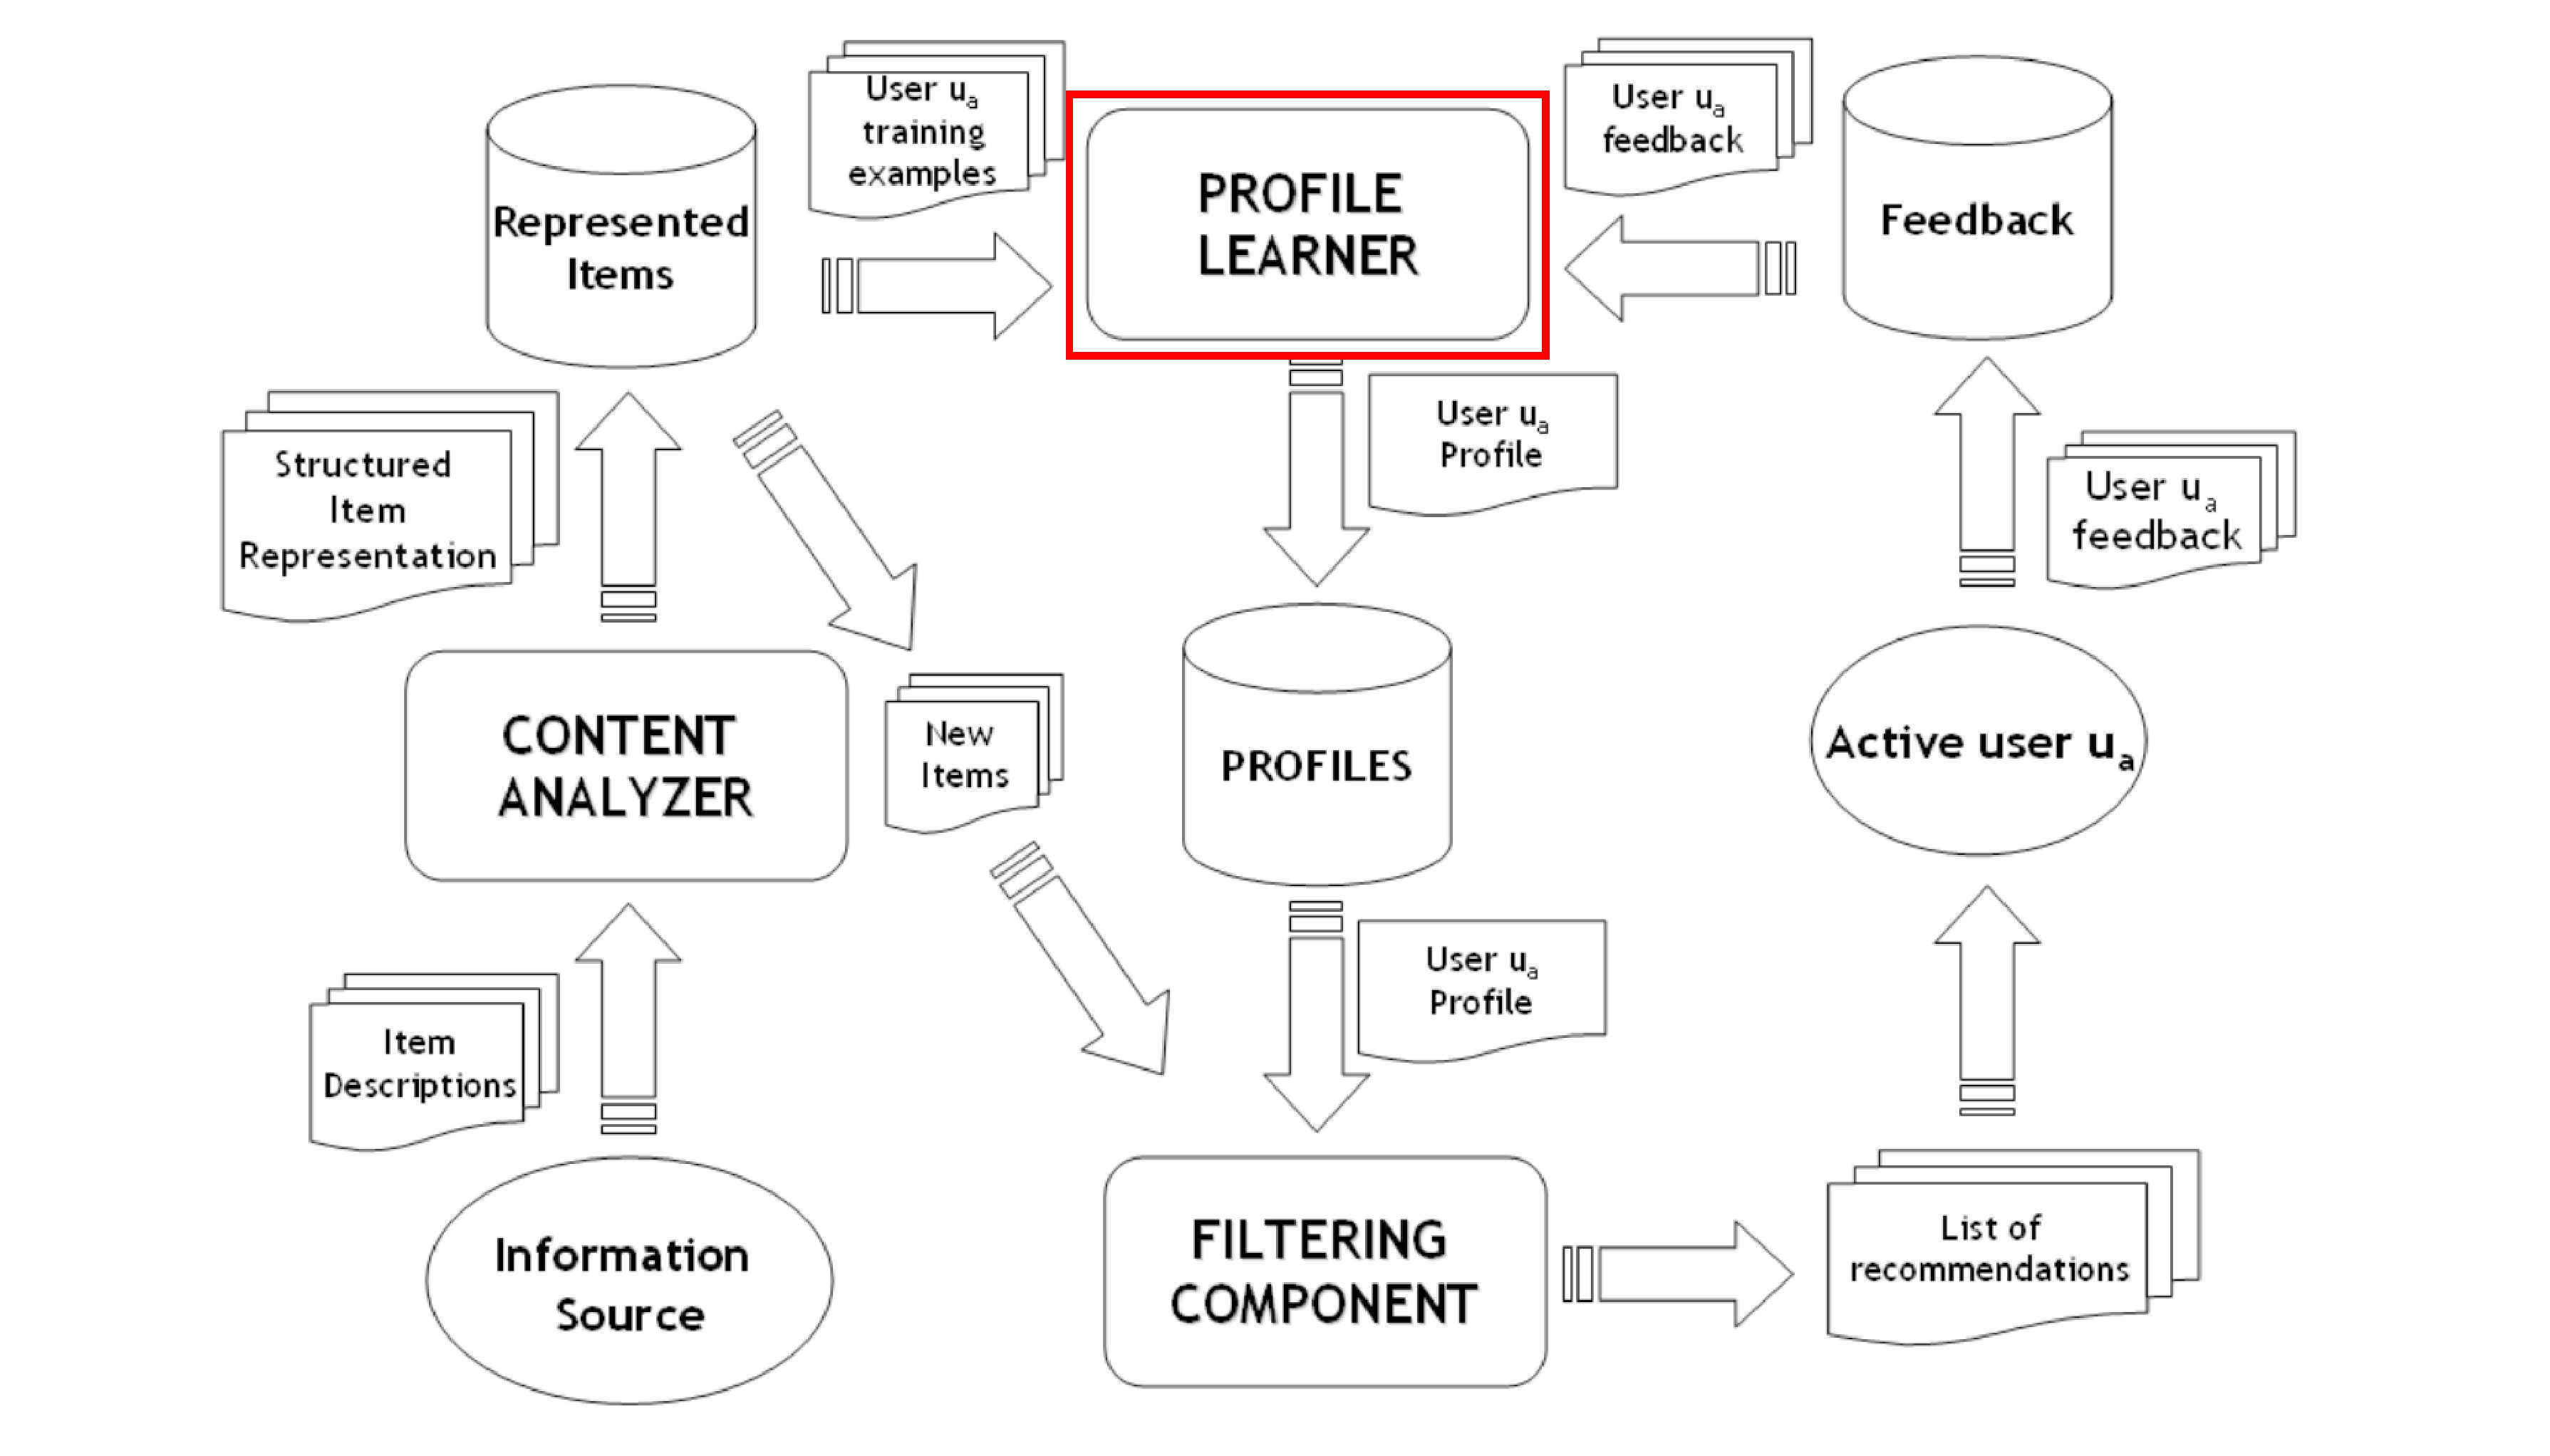
\includegraphics[width=1\textwidth]{figura/recomendacao_conteudo_3.eps}
  \caption{Fluxo para construção de um sistema de recomendação por conteúdo (LOPS; GEMMIS; SEMERARO, 2011)}
\end{figure}

\end{frame}

\begin{frame}

\begin{figure}[h!]
  \centering
    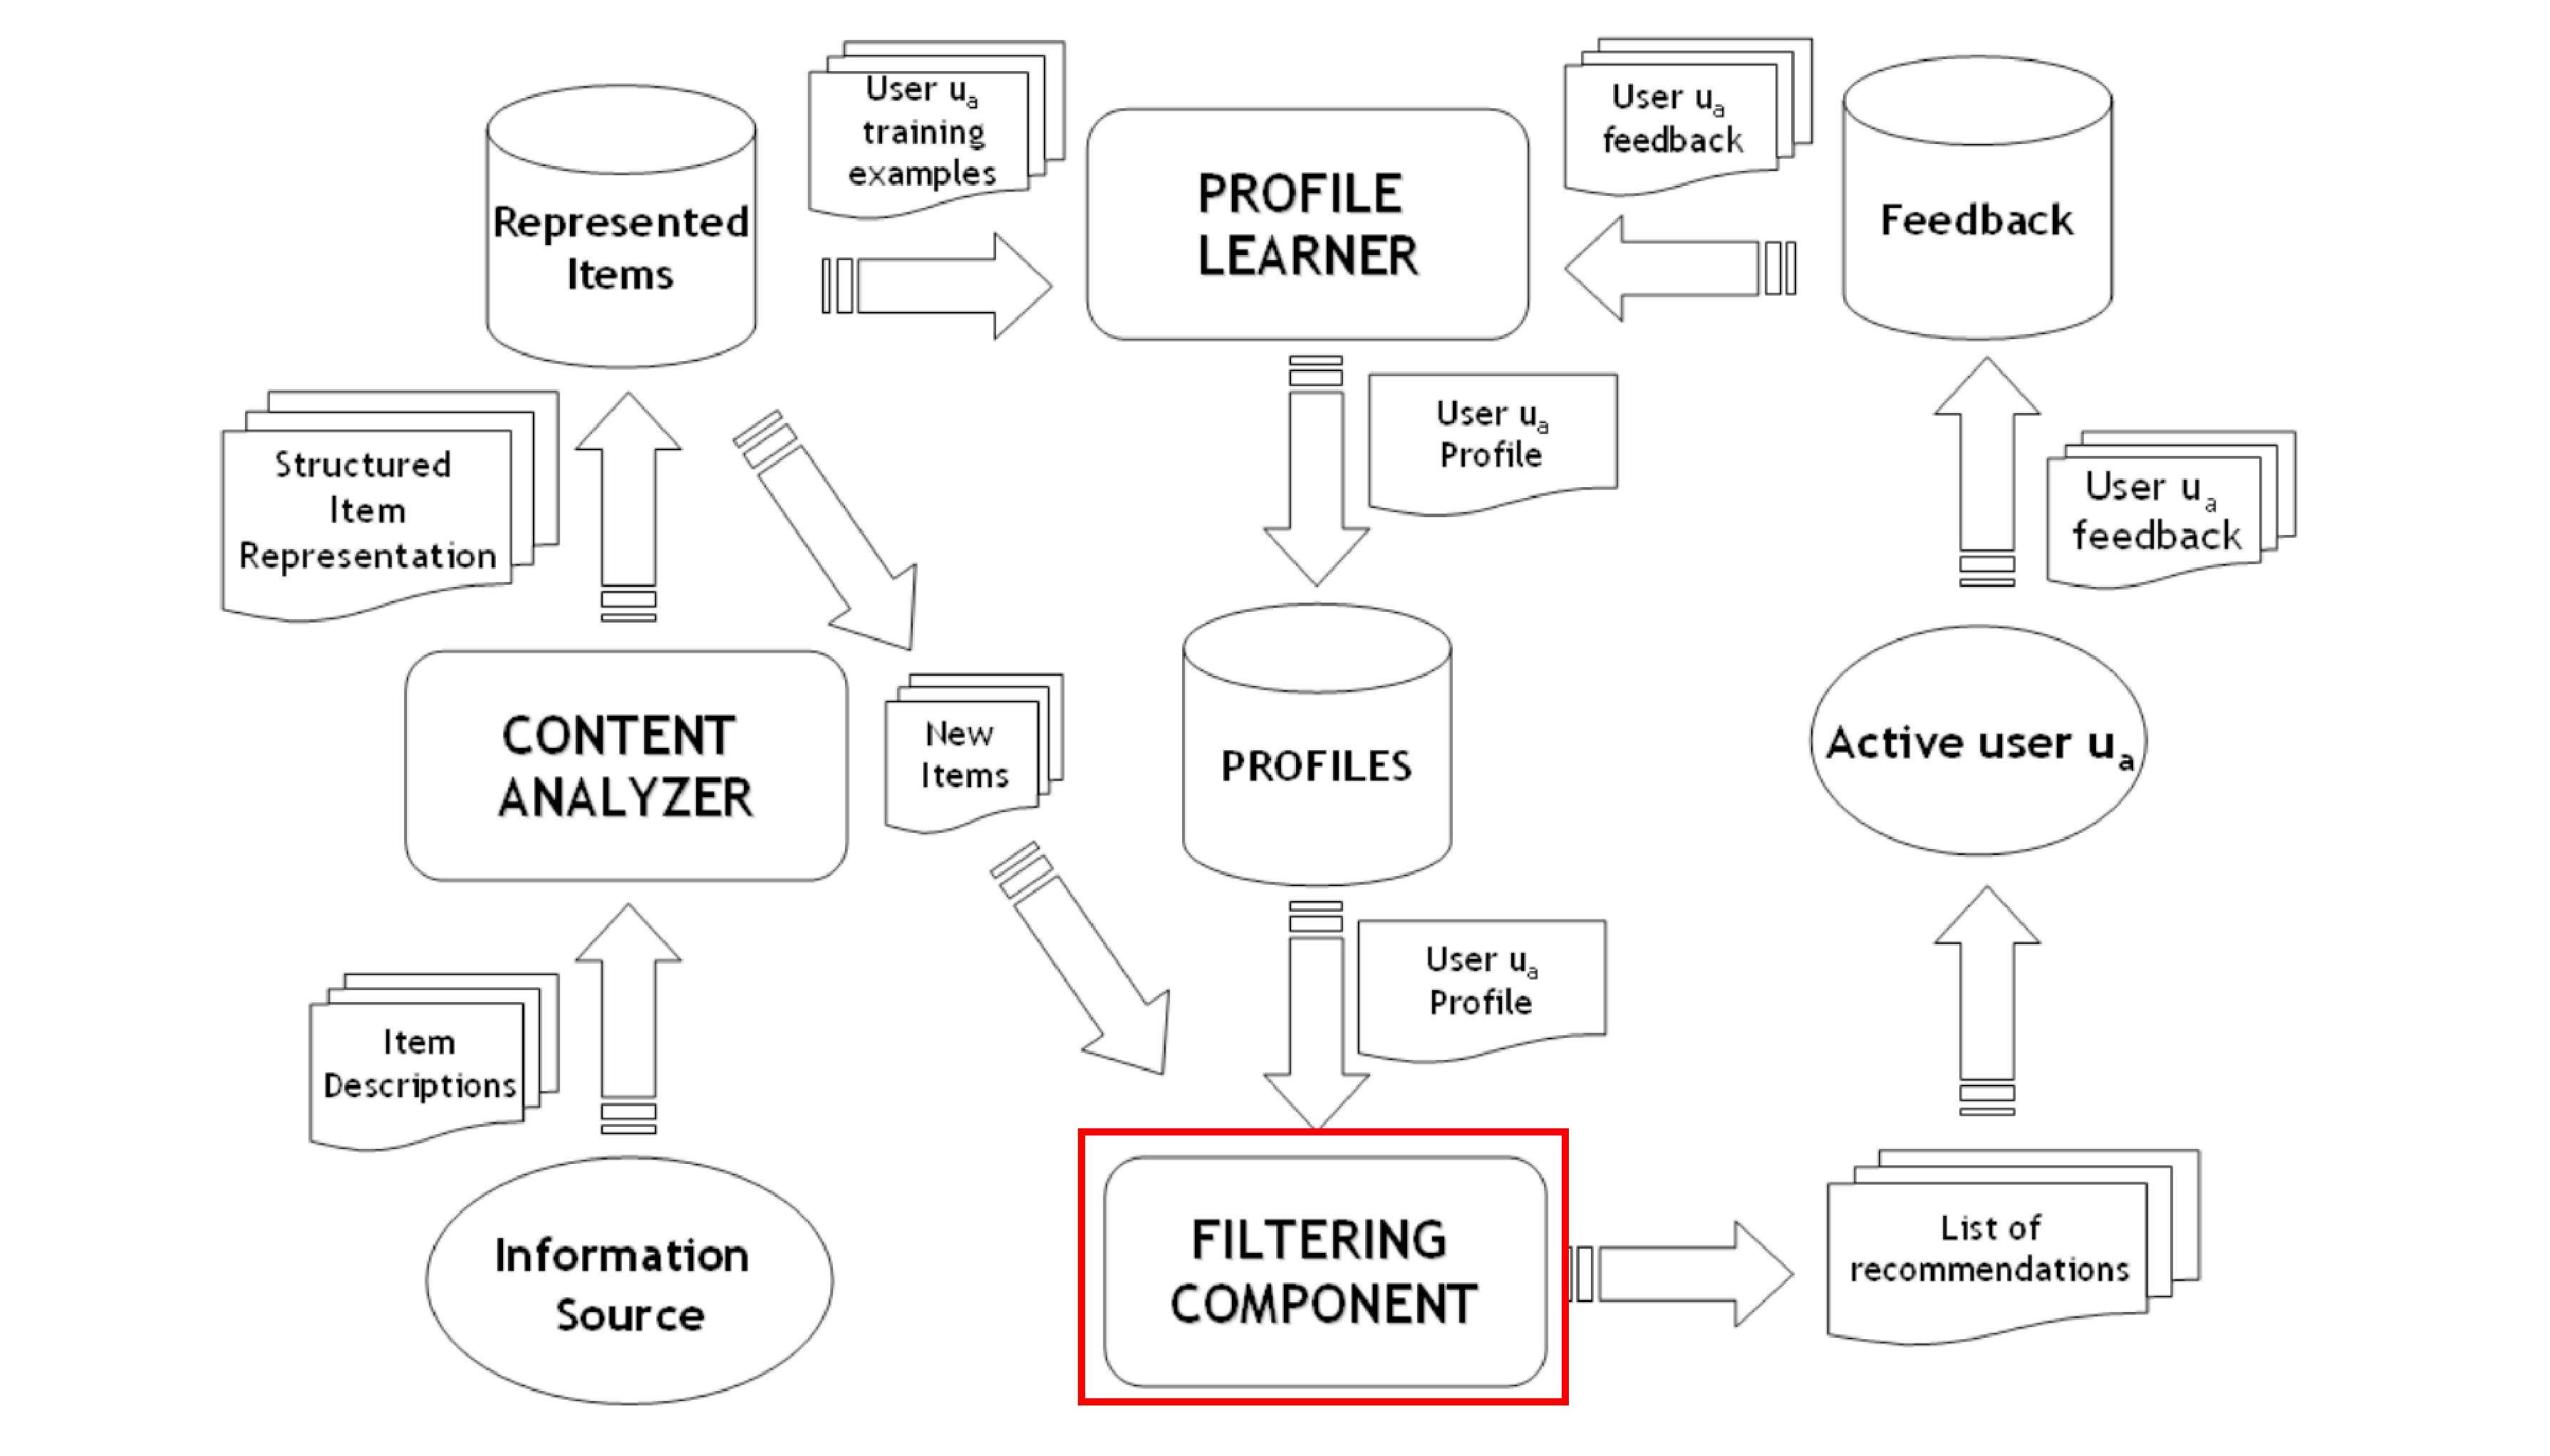
\includegraphics[width=1\textwidth]{figura/recomendacao_conteudo_4.eps}
  \caption{Fluxo para construção de um sistema de recomendação por conteúdo (LOPS; GEMMIS; SEMERARO, 2011)}
\end{figure}

\end{frame}

\begin{frame}

\begin{figure}[h!]
  \centering
    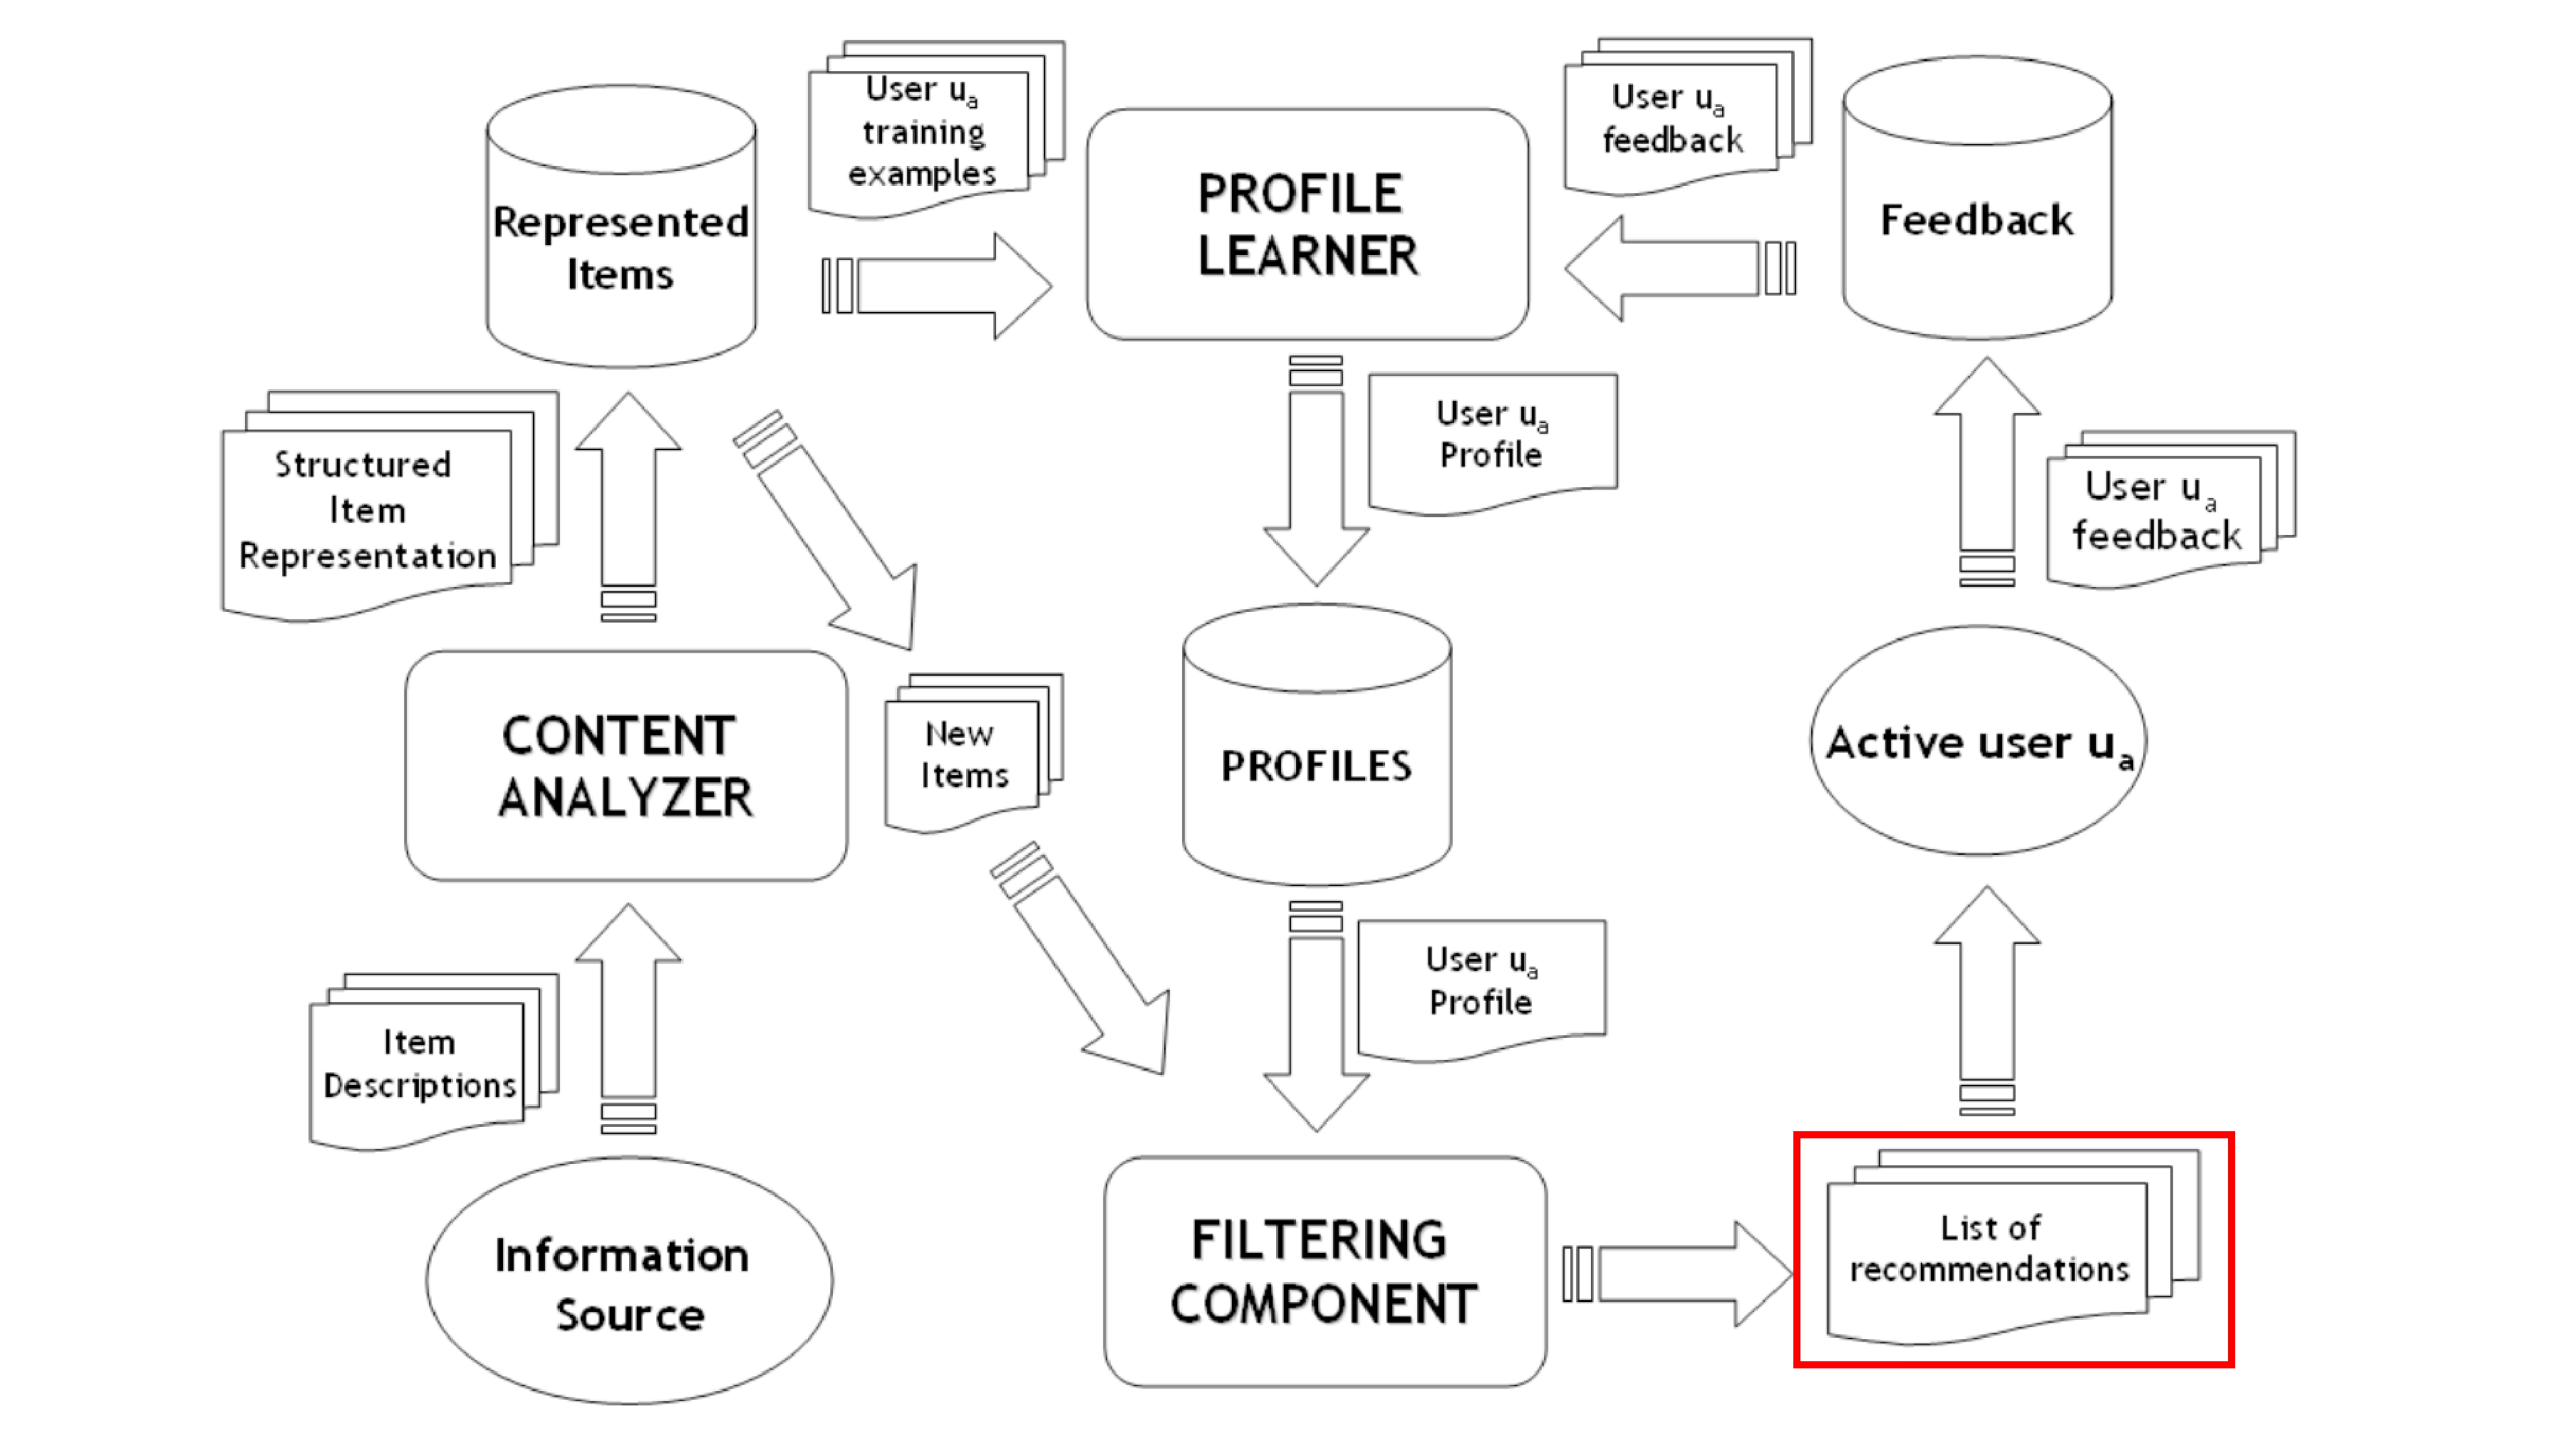
\includegraphics[width=1\textwidth]{figura/recomendacao_conteudo_5.eps}
  \caption{Fluxo para construção de um sistema de recomendação por conteúdo (LOPS; GEMMIS; SEMERARO, 2011)}
\end{figure}

\end{frame}

\begin{frame}

\begin{figure}[h!]
  \centering
    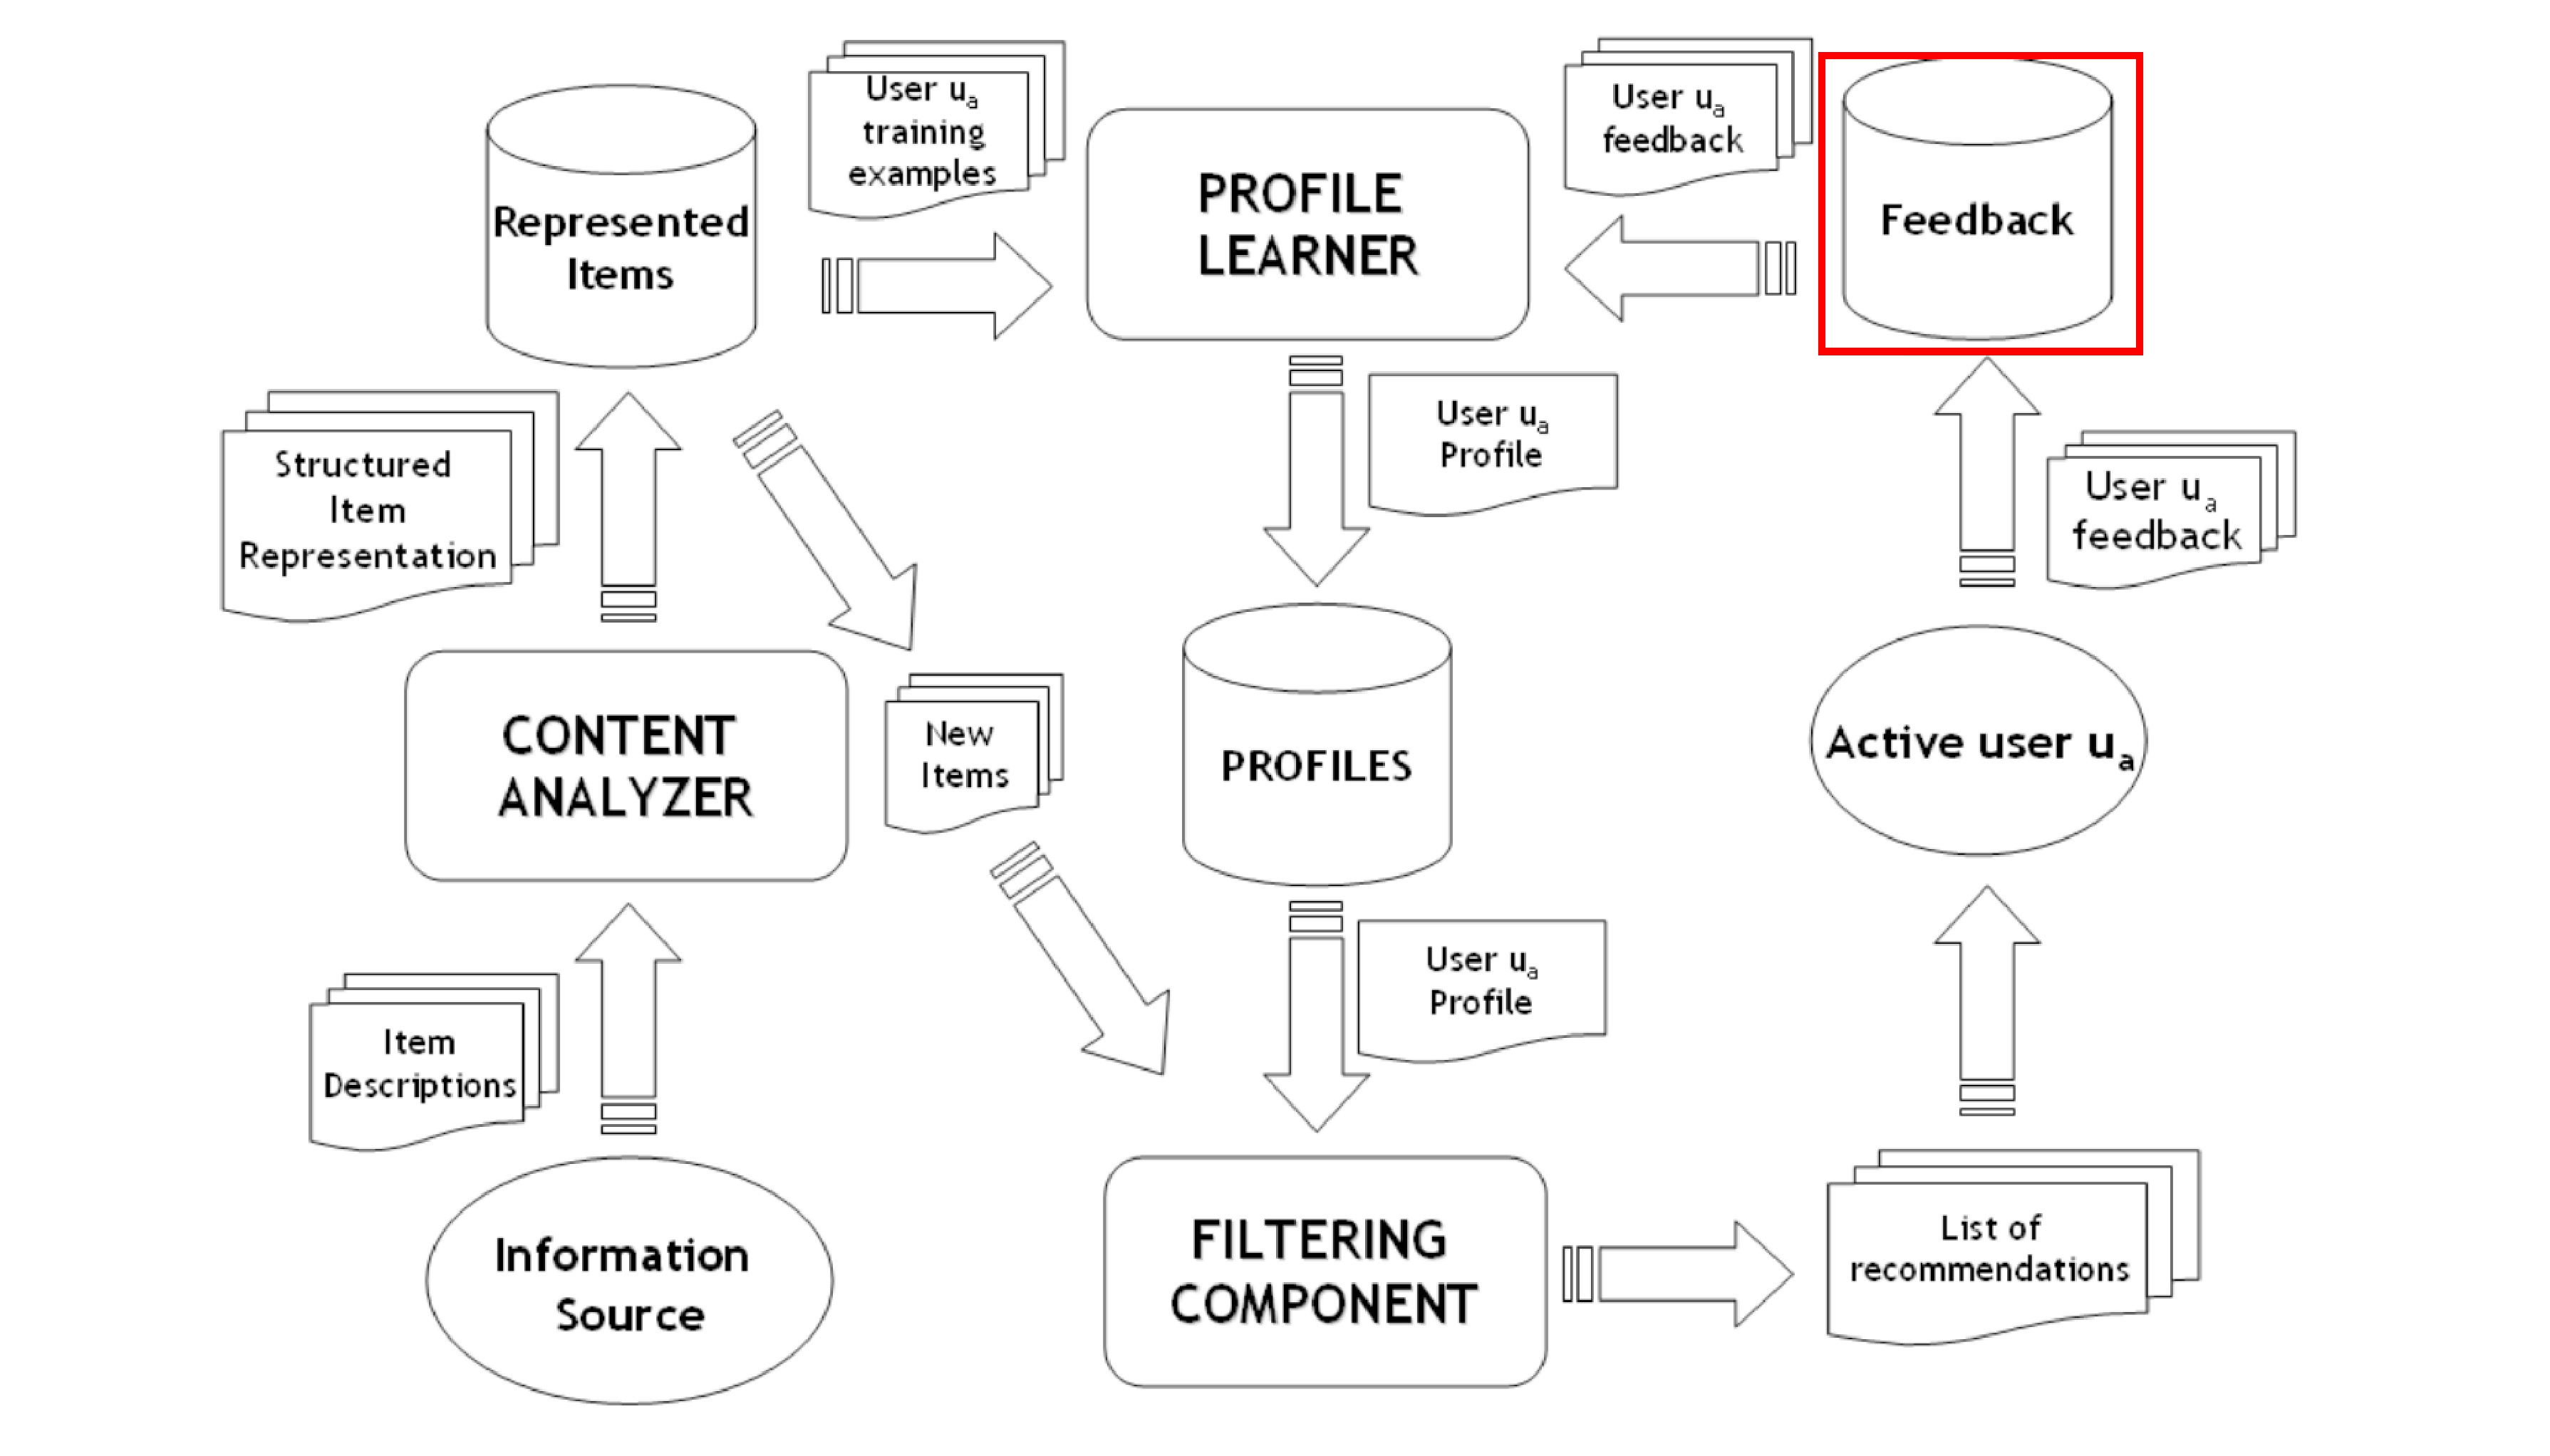
\includegraphics[width=1\textwidth]{figura/recomendacao_conteudo_6.eps}
  \caption{Fluxo para construção de um sistema de recomendação por conteúdo (LOPS; GEMMIS; SEMERARO, 2011)}
\end{figure}

\end{frame}


% section l (end)

\section{Software escolhido} % (fold)
\label{sec:software_escolhido}
\begin{frame}
\begin{itemize}
    \item AppRecommender

    \item \say{\textit{dada a lista de programas instalados em determinado sistema,
          o recomendador retorna uma lista de aplicativos sugeridos, que supostamente
          são aplicativos de potencial interesse para os usuários daquele sistema}}, \\ARAÚJO, T. C
\end{itemize}
\end{frame}

\begin{frame}
    Perfil de Usuário

\begin{itemize}
    \item Lista de termos mais significativos para o usuário
    \item Um termo pode ser uma debtag ou um
    \item Uma estratégia de recomendação seleciona esses termos
\end{itemize}
\end{frame}

\begin{frame}
\begin{figure}[h]
  \centering
  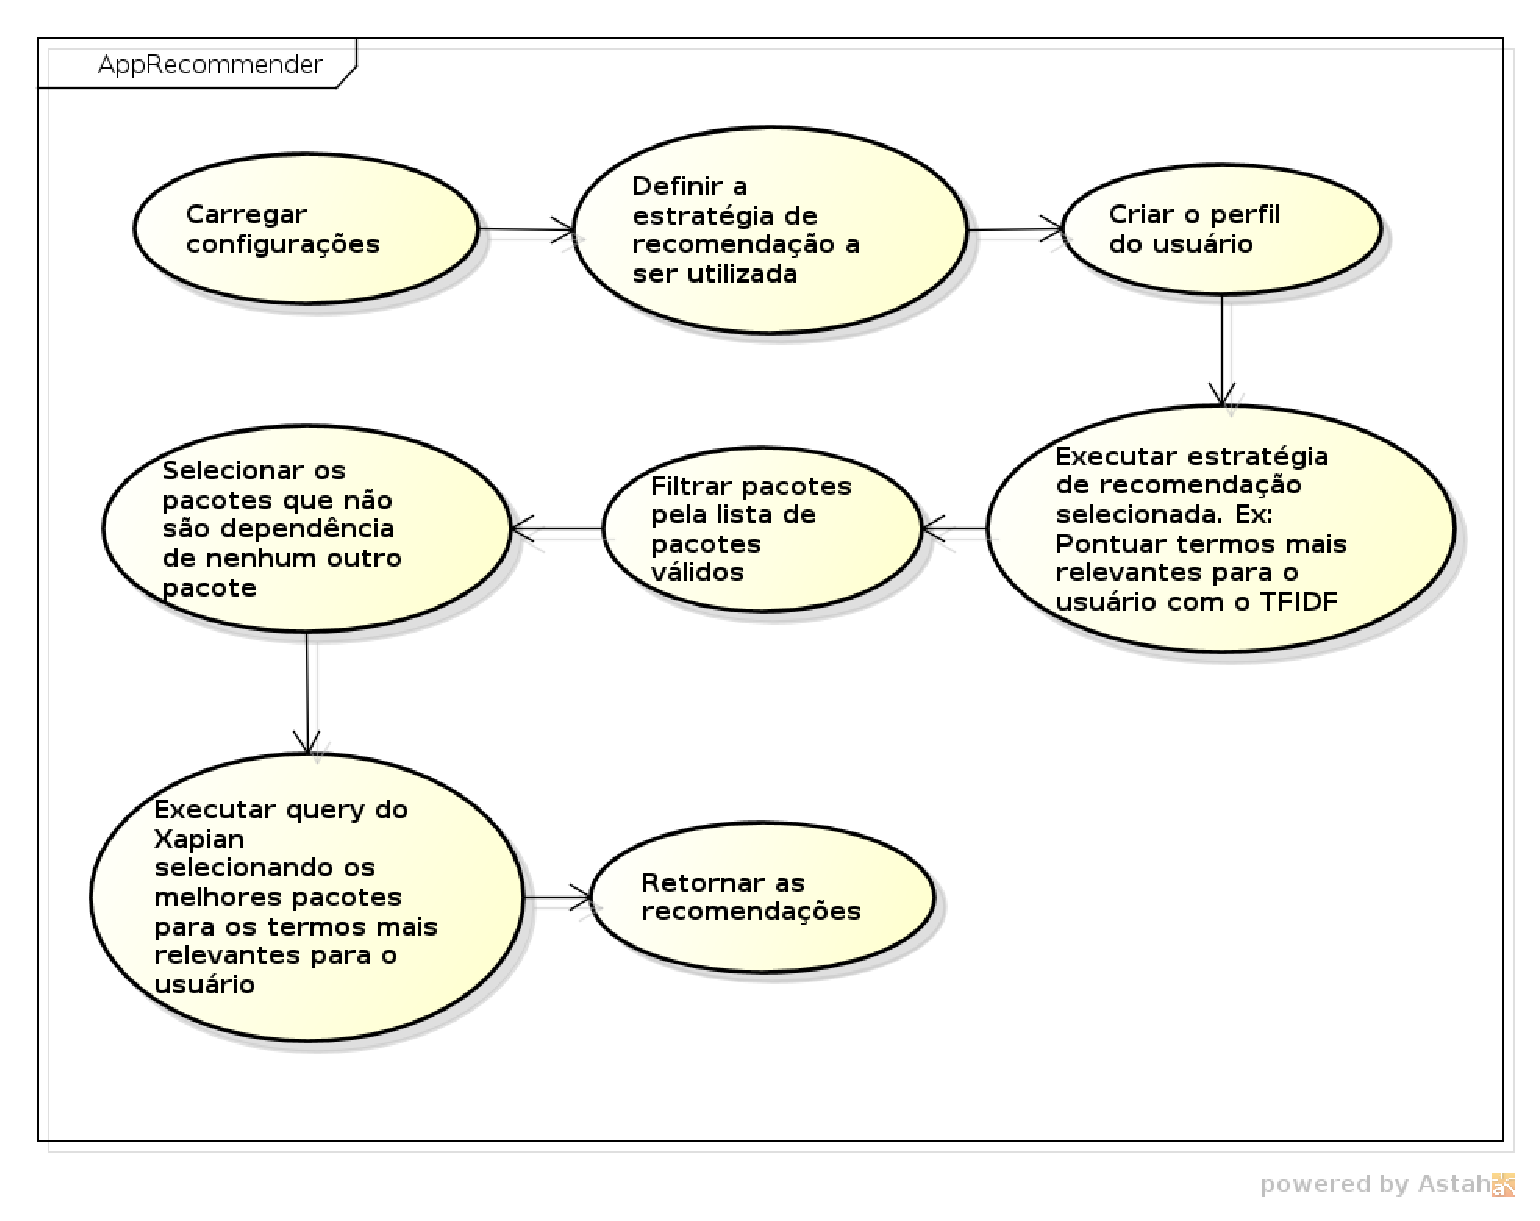
\includegraphics[width=0.9\textwidth]{figura/app_recommender_process.eps}
  \caption{Processo do AppRecommender}
  \label{fig:curva_aprendizado}
\end{figure}
\end{frame}

\section{Contexto temporal no Debian} % (fold)
\label{sec:d}

\begin{frame}

    \begin{itemize}
        \item Stat
        \item Popularity-contest
    \end{itemize}

\end{frame}

\begin{frame}
\begin{figure}[h!]
    \centering
    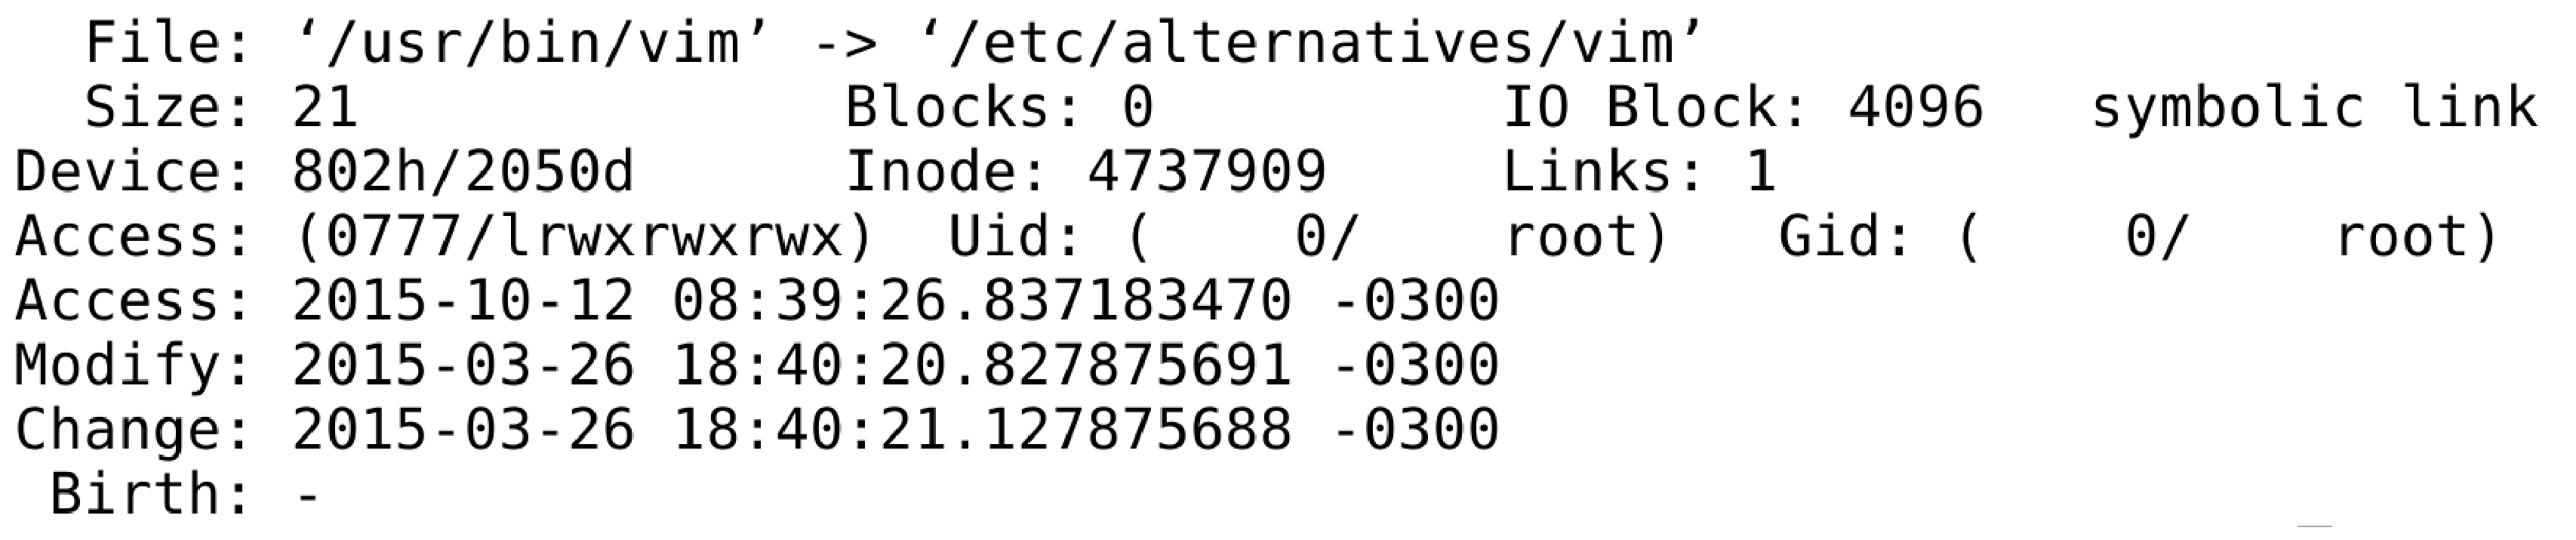
\includegraphics[width=1\textwidth]{figura/comando_stat.eps}
    \caption{Saída do comando stat para um dado software}
\end{figure}
\end{frame}


\begin{frame}
\begin{figure}[h!]
    \centering
    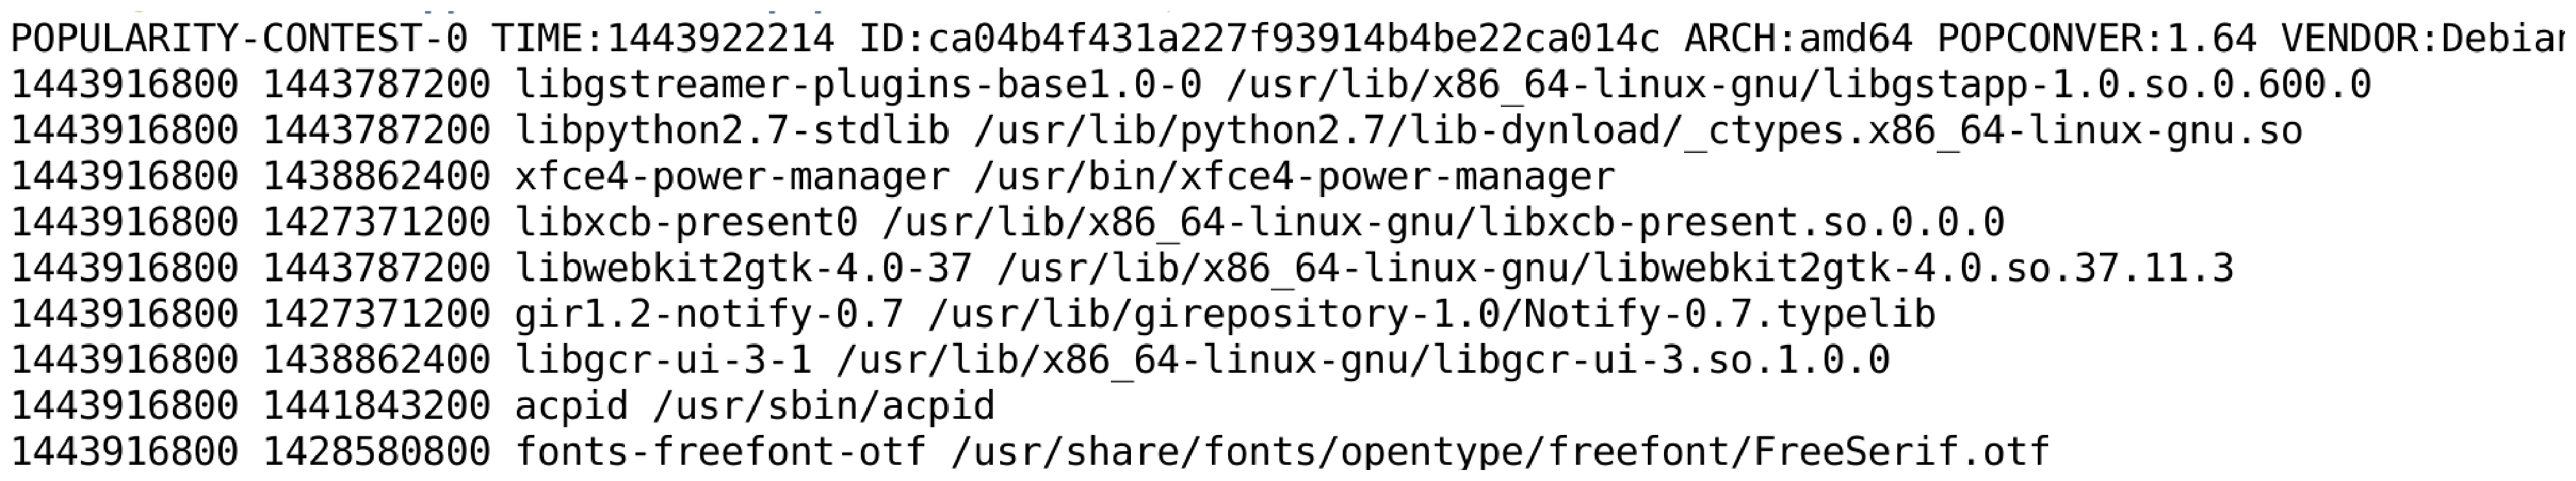
\includegraphics[width=1\textwidth]{figura/popularity_contest.eps}
    \caption{Saída do popularity-contest para um dado usuário}
\end{figure}
\end{frame}


\begin{frame}

Fórmula usada para gerar um valor de contexto temporal para um dado pacote:
\newline
\newline
ClassificaçãoTempo = $\frac{TempoAcesso - TempoModificação}{TempoAtual -
TempoModificação}$

\end{frame}


\begin{frame}
    Restrição quanto ao sistema de arquivo

    \begin{itemize}
        \item noatime
        \item stricatime
        \item relatime
    \end{itemize}
\end{frame}

\begin{frame}

    \begin{itemize}
        \item Pacotes usados sem intervenção direta do usuário
            \begin{itemize}
                \item Retirada de pacotes com prioridade \textit{Required},
                      \textit{Important} e \textit{Standard}.
            \end{itemize}
        \item Flag relatime não apresenta valores exatos
    \end{itemize}

\end{frame}

% section d (end)
\section{Estratégia determinística} % (fold)
\label{sec:estrategia_deterministica}

\begin{frame}
\begin{itemize}
    \item Utiliza do mesmo processo do AppRecommender
    \item Modifica o cálculo do peso dos pacotes em uma estratégia
    baseada em conteúdo
    \item O peso do pacote é resultado do produto do TFIDF com o
    Peso Temporal do pacote
\end{itemize}
\end{frame}

\begin{frame}
\begin{itemize}
    \item O peso de um termo é calculado pela média aritimética dos cinco
pacotes com maiores pesos que estão associados
ao termo.
    \item Caso o termo possua menos de 5 pacotes os valores faltantes são
preenchidos pelo peso anterior com um decréscimo de 0.05
\end{itemize}
\end{frame}

\begin{frame}
\begin{itemize}
    \item \textbf{PesoPacote} = C / $\exp\left(-({1 - ClassificaçãoTempo}) * {\lambda}\right)$
    \item Onde C e ${\lambda}$ são constantes usadas para alterar a velocidade do
decaimento da curva e o peso dado a variável \textit{ClassificaçãoTempo}.
\end{itemize}
\end{frame}

\begin{frame}
    $ValorTemporalDoTermo = \frac{1}{5} * \sum\limits_{i=1}^{5} [Peso Dos Pacotes Ordenados]$
\end{frame}

\begin{frame}
    $PesoDoTermo = TFIDF * ValorTemporalDoTermo$
\end{frame}

% section d (end)

\section{Aprendizado de máquina} % (fold)

\begin{frame}

    \begin{itemize}
        \item Estratégia de pós-filtragem
        \item Rótulos do pacote
        \item Formatação dos dados
        \item Estratégia de aprendizado
    \end{itemize}

\end{frame}

\begin{frame}

    Rótulos do pacote:
    \newline
    \newline

    \begin{table}[h]
    \centering
    \begin{tabular}{cc}
    \hline
    \rowcolor[HTML]{EFEFEF}
    {Escala} & {Valores} \\ \hline
    {Excelent(EX)}  & ClassificaçãoTempo >= 0.8                  \\ \hline
    {Great(G)}   & ClassificaçãoTempo >= 0.7                  \\ \hline
    {Medium(M)}   & ClassificaçãoTempo >= 0.5                  \\ \hline
    {Bad(B)}   & ClassificaçãoTempo >= 0.3                  \\ \hline
    {Horrible(H)}   &ClassificaçãoTempo < 0.3                   \\ \hline
    \end{tabular}
    \caption{Escala para classificação de um pacote baseado em seus atributos de tempo}
    \label{tab:classificacao_pacotes}
    \end{table}

\end{frame}

\begin{frame}

    \begin{itemize}
        \item Vetores binários para representar um pacote
        \item Debtags e descrição do pacote
        \item Termos usados apenas dos pacotes manualmente instalados pelo
              usuário
    \end{itemize}
\end{frame}

\begin{frame}

    \begin{itemize}
        \item Bayes ingênuo
        \item Uso da probabilidade de bayes
        \item Distribuição de Bernoulli
        \item Dependência entre variáveis não levada em conta
        \item Linearização do método
    \end{itemize}

\end{frame}

\begin{frame}

    Fórmula adotada para o bayes ingênuo:
    \newline
    \newline
    $Classificador = max(p(C_{y})*\prod_{i=1}^{N}p(x_{i}|C_{y}))$

\end{frame}

\begin{frame}

    \begin{itemize}
        \item Validação cruzada
        \item Curvas de Aprendizado
    \end{itemize}

\end{frame}

\begin{frame}

\begin{figure}[h]
  \centering
  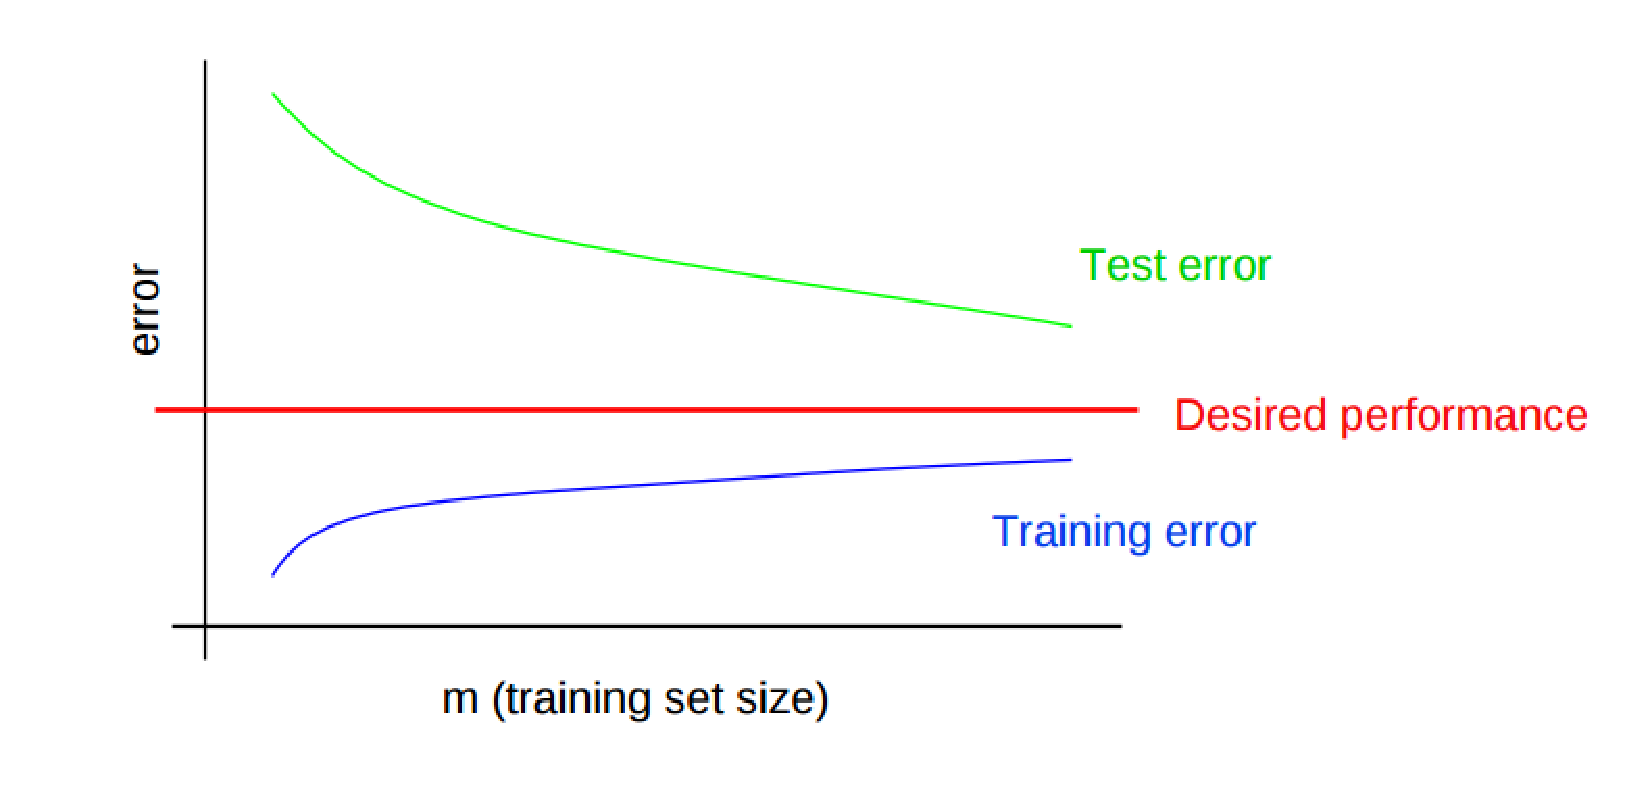
\includegraphics[width=0.9\textwidth]{figura/curva_aprendizado.eps}
  \caption{Exemplo de uma curva de aprendizado}
  \label{fig:curva_aprendizado}
\end{figure}

\end{frame}


\label{sec:aprendizado_maquina}

\section{Comparação dos resultados} % (fold)
\label{sec:comparacao_resultados}

\begin{frame}
    \begin{itemize}
        \item Comparação baseadas no \textit{AppRecommender}
        \item Foco em precisão e novidade das recomendações
        \item Comparação \textit{offline}
        \item Teste com usuário
    \end{itemize}
\end{frame}

\begin{frame}
\begin{figure}[h]
  \centering
  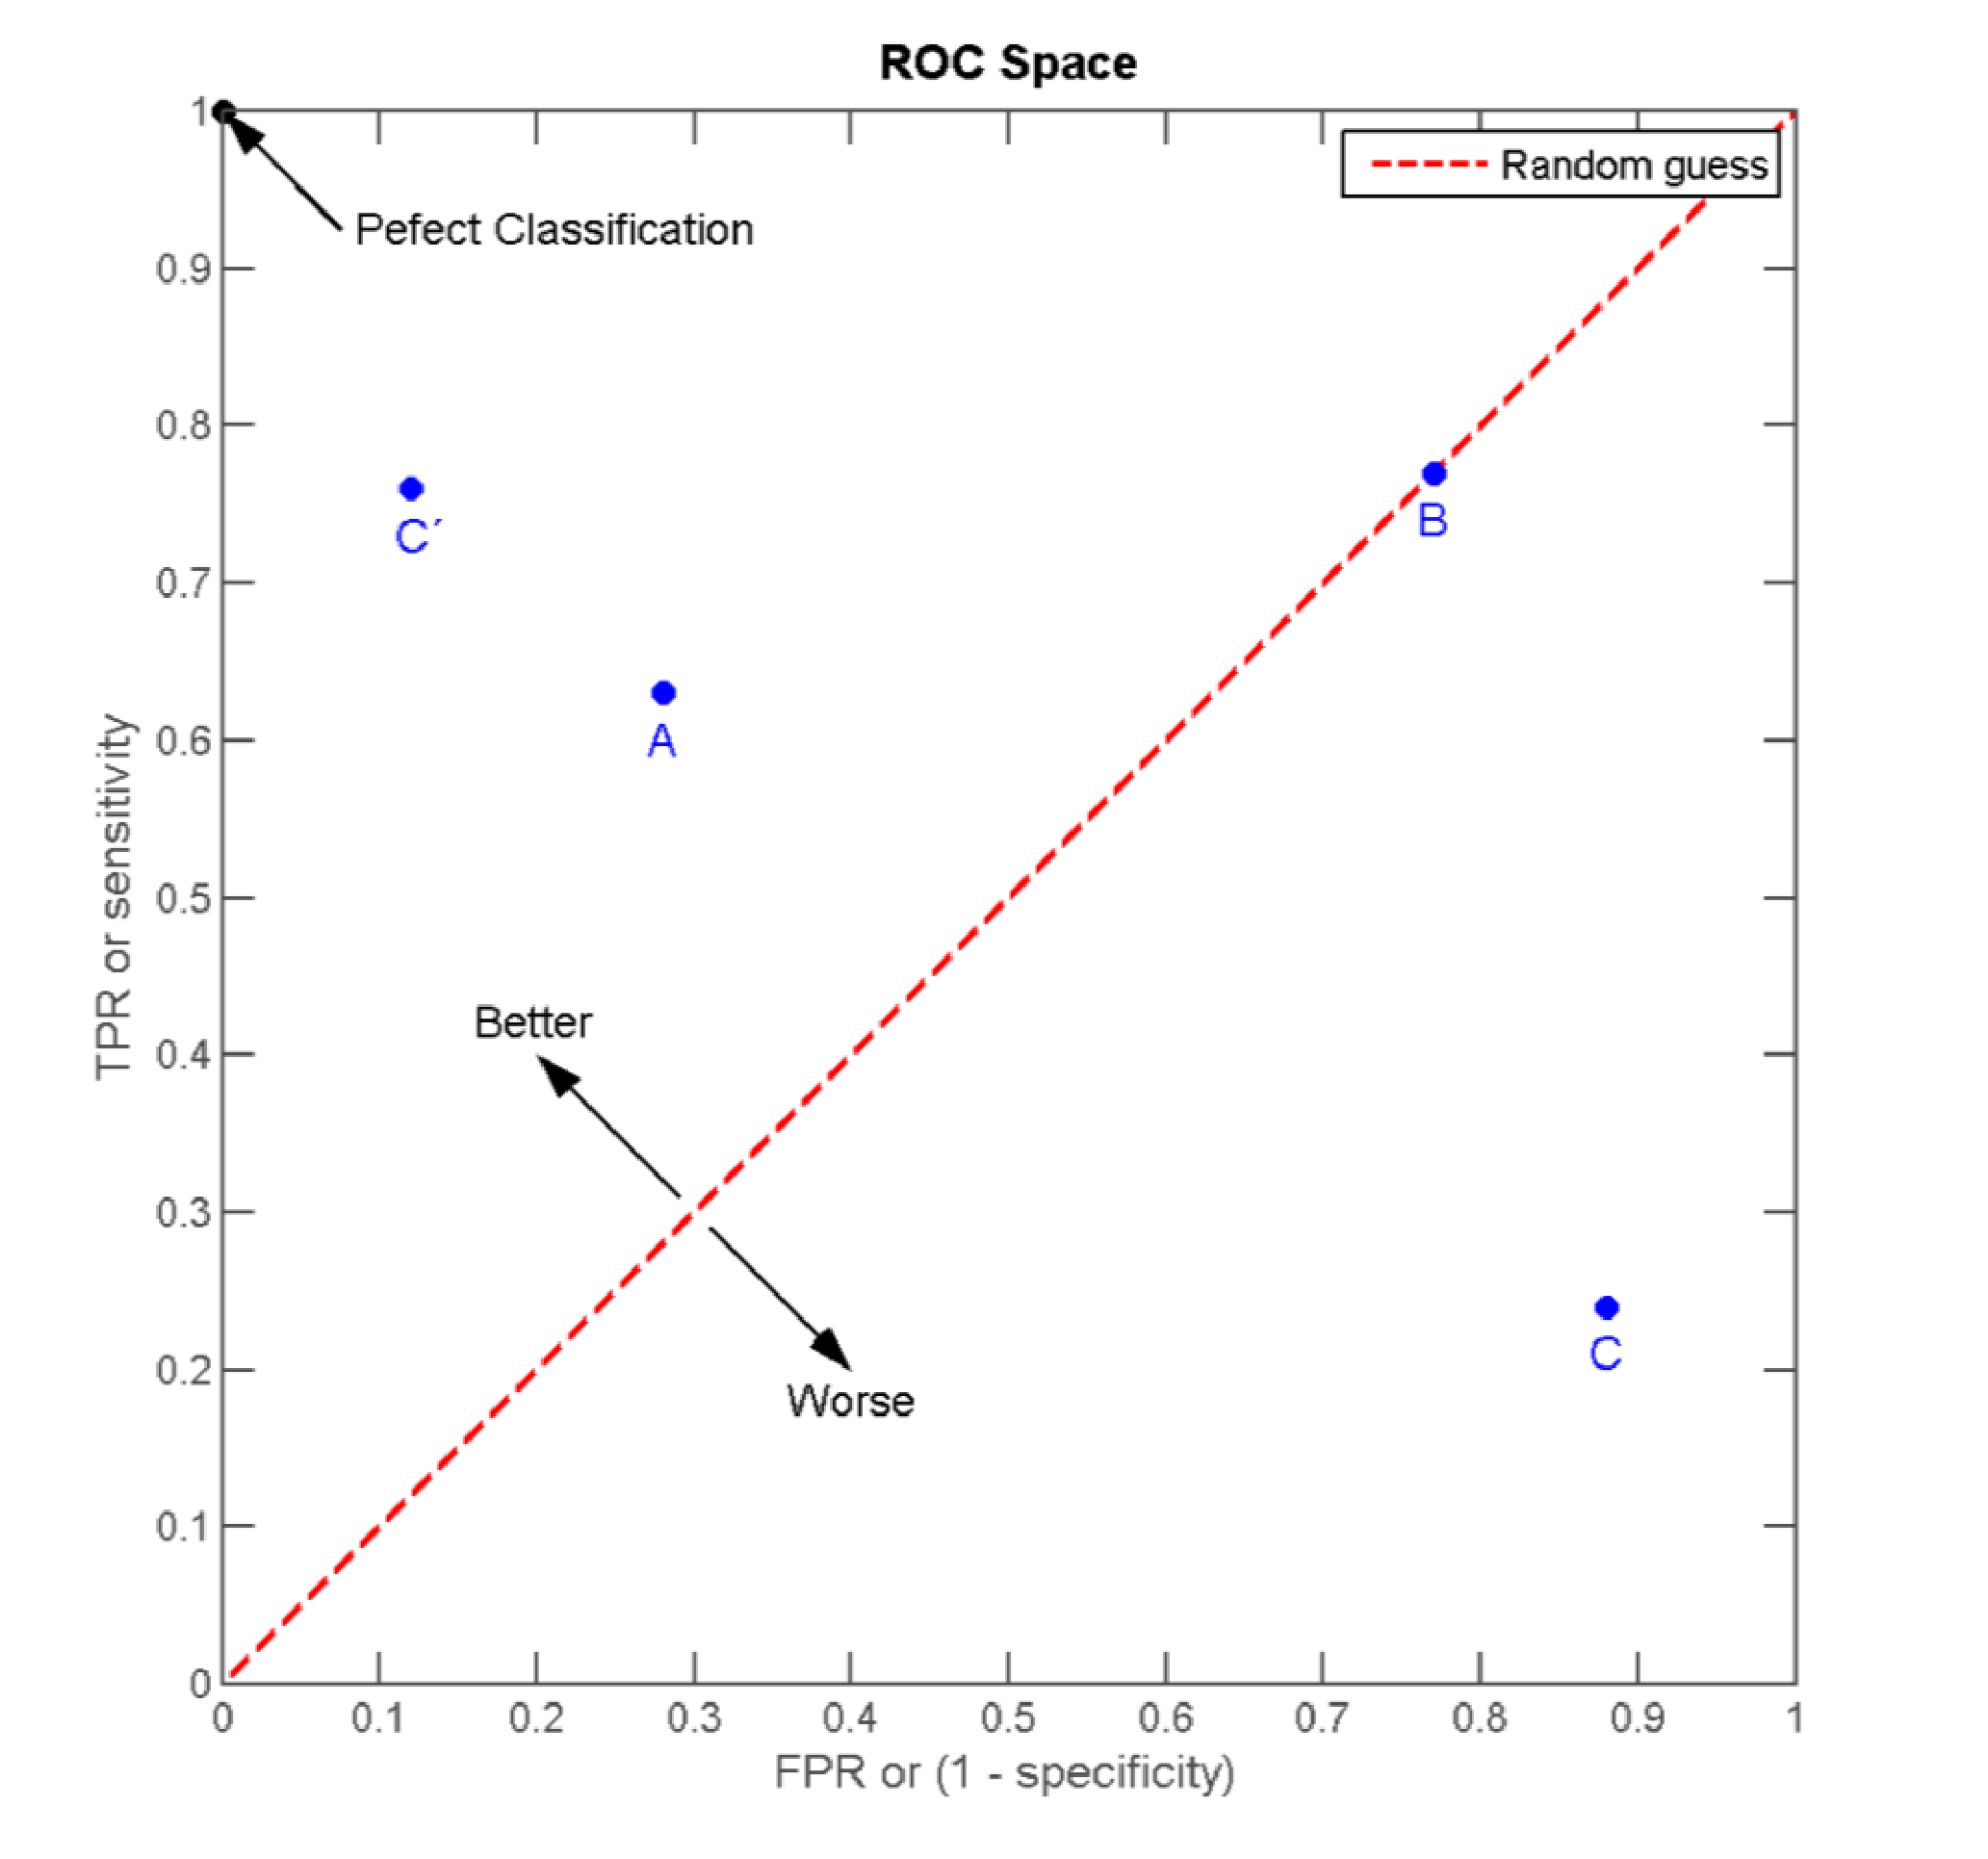
\includegraphics[width=0.7\textwidth]{figura/curva_roc.eps}
  \caption{Exemplo de curva ROC}
  \label{fig:curva_roc}
\end{figure}

\end{frame}

\begin{frame}

    \begin{itemize}
        \item Usuário será apresentado a 5 recomendações de cada vez
        \item 4 estratégias distintas
        \item 20 recomendações de pacotes no total
    \end{itemize}

\end{frame}

\begin{frame}

 \begin{itemize}
    \item \textbf{Ruim: } Recomendação que não agrada ao usuário.
    \item \textbf{Redundante: } Usuário possui aplicativos similares para o item
        sendo recomendado.
    \item \textbf{Útil: } Usuário acha que a recomendação lhe proporciona um
            pacote útil.
    \item \textbf{Surpresa boa: } Usuário considera a recomendação útil e além
        do mais inesperada.
\end{itemize}


\end{frame}

\begin{frame}

\begin{itemize}
    \item \textbf{Precisão: } $\frac{VerdadeirosPositivos}{VerdadeirosPositivos
        + FalsoNegativos}$
    \item \textbf{Novidade: } $\frac{NumSurpresaBoa}{VerdadeirosPositivos +
        FalsoNegativos}$
\end{itemize}

Onde:

    \begin{itemize}
        \item VerdadeirosPositivos: Útil e Surpresa boa
        \item FalsoNegativos: Ruim e Redundante
    \end{itemize}

\end{frame}

\section{Resultados parciais} % (fold)
\label{sec:resultados_parciais}

\section{Obrigado!}
\label{sec:obrigado}


